% FINAL_MANUSCRIPT.tex — journal-ready production of the accepted manuscript
% Task-13 presentation upgrade (2026-09-07): expanded verified bibliography,
% subsectioned introduction, figure-by-figure physical interpretation,
% structured discussion. Science, numbers, and equations unchanged from the
% accepted (frozen) formulation.
% Target: Applied Mathematics and Mechanics (English Edition) structure
% (publisher class file applied at portal submission; structure, numbering,
%  and reference style are compliant)
\documentclass[11pt]{article}
\usepackage[margin=2.6cm]{geometry}
\usepackage{amsmath,amssymb}
\usepackage{graphicx}
\graphicspath{{../figures/output/}{figures/}}
\usepackage{booktabs}
\usepackage{caption}
\usepackage{array}
\captionsetup{font=small,labelfont=bf}
\usepackage[colorlinks=true,linkcolor=blue,citecolor=blue,urlcolor=blue]{hyperref}
\newcommand{\dd}{\mathrm{d}}
\newcommand{\e}{\varepsilon}
\newcommand{\om}{\omega}
\newcommand{\Om}{\Omega}
\newcommand{\sig}{\sigma}
\newcommand{\tht}{\theta}
\newcommand{\Dw}{D_w}
\newcommand{\rw}{\rho_w}

\title{\bf Surface waves in a two-dimensional hexagonal piezoelectric thermoelastic quasicrystal half-space: a semi-analytical study of inertial, diffusive, and telegraph-type phason dynamics}

\author{[AUTHOR INFORMATION TO BE INSERTED]\\
\small [AFFILIATIONS TO BE INSERTED]\\
\small Corresponding author: [NAME, E-MAIL, ORCID TO BE INSERTED]}
\date{}

\begin{document}
\maketitle

\begin{abstract}
\noindent Surface-wave propagation in a two-dimensional (2D) hexagonal quasicrystal half-space is analysed within a linear piezoelectric--thermoelastic formulation that treats the phonon and phason degrees of freedom on equal footing. The active sagittal problem couples the phonon displacements $(u_x,u_z)$, the phason displacements $(w_x,w_z)$, and the temperature increment $\tht$; in the studied configuration (propagation along a two-fold axis, periodic direction inert) the electric potential decouples exactly and enters only as a passive output. Three phason dynamic models are compared: an inertial model (A, $\rw\ddot w=\mathrm{div}\,H$), a diffusive model (B, $\Dw\dot w=\mathrm{div}\,H$), and a telegraph-type model (C, $\rw\ddot w+\Dw\dot w=\mathrm{div}\,H$), with Lord--Shulman thermal relaxation. The surface-wave problem is reduced, without spatial discretisation of the half-space, to a $5\times5$ boundary matrix $B(\om,k)$ assembled from the five decaying depth roots of a tenth-degree matrix pencil $M(\om,k,p)=A_0+pA_1+p^2A_2$; the secular condition is monitored through the scale-explicit indicator $r=\sigma_{\min}(B)/\lVert B\rVert$. After verification against classical elastic limits, symbolic identities, and the model limits C$\to$A and C$\to$B, the production sweeps show: (i)~at baseline friction the phason-dominated branch of model A ($V^*\approx0.3107$, phason participation $P_w\approx0.99$) is separated by $\Delta_{AC}\approx0.33$ from the phonon--Rayleigh branches of models B and C ($V^*\approx0.4663$), whereas B and C are mutually indistinguishable over 95 of 121 grid points within a benchmarked numerical-resolution floor $\e_\Delta=1.13\times10^{-8}$; (ii)~when the phason friction $D_w^*$ is controlled, the B--C difference becomes resolvable (up to $5.0\times10^{-3}$ relative) in a region of the $(\Om,D_w^*)$ plane that slides with $D_w^*$, while at the baseline $D_w^*$ the two models remain indistinguishable almost everywhere; (iii)~thermal relaxation (sweep in $\tau_0^*$) produces a weak but resolvable effect, $\max\Delta_T=7.9\times10^{-5}$, at the largest relaxation time; (iv)~clamping the phason at the surface changes the model-C wave speed by at most $8.1\times10^{-6}$ relative, and destroys the model-A surface branch altogether. Physically, the results indicate that the phason dynamic class controls \emph{which} surface branch exists --- inertial phasons carry a distinct slow surface mode, whereas dissipative phasons are slaved to the phonon--Rayleigh branch --- while the diffusive/telegraph distinction is observable only when the phason friction is low (or the frequency high) relative to the phason inertia. The findings are statements about the declared composite/surrogate parameter set, bounded by the numerical resolution floor; no experimental validation is claimed, and no claim beyond the investigated parameter ranges is made. All computations are nondimensional, deterministic, and reproducible from the accompanying reproducibility package.

\vspace{4pt}
\noindent\textbf{Keywords:} quasicrystal; phason dynamics; surface waves; Rayleigh waves; piezoelectricity; Lord--Shulman thermoelasticity; telegraph equation; semi-analytical method

\vspace{2pt}
\noindent\textbf{Mathematics Subject Classification (2020):} 74J15; 74F05; 74F15; 52C23
\end{abstract}

\section*{Nomenclature (principal symbols)}
{\small
\begin{center}
\begin{tabular}{ll@{\hspace{1.2cm}}ll}
$u_i$ & phonon displacement & $w_i$ & phason displacement \\
$\e_{ij}$ & phonon strain & $w_{ij}=\partial_j w_i$ & phason displacement gradient \\
$\sig_{ij}$ & phonon stress & $H_{ij}$ & phason pseudo-stress \\
$\tht=T-T_0$ & temperature increment & $\tau_0$ & Lord--Shulman relaxation time \\
$\rho,\ \rw$ & phonon, phason inertia & $\Dw$ & phason friction \\
$k,\ p$ & surface, depth wavenumbers & $\om$ & angular frequency \\
$k_0,\ v_0,\ \om_0$ & reference scales & $(\cdot)^*$ & nondimensional quantity \\
$\Om=\om/\om_0$ & nondimensional frequency & $V^*=\Om/k^*$ & nondimensional phase speed \\
$B(\om,k)$ & $5\times5$ surface matrix & $r=\sigma_{\min}(B)/\lVert B\rVert$ & secular indicator \\
$\delta^*=1/|\mathrm{Im}\,p|$ & penetration depth & $P_w$ & phason participation \\
$\e_\Delta$ & resolution floor & $\Om_c=\Dw^*/\rw^*$ & phason crossover frequency \\
\end{tabular}
\end{center}}

\section{Introduction}

\subsection{Quasicrystals and the phason degree of freedom}

Quasicrystals are solids with long-range orientational order, sharp diffraction, and rotational symmetries --- fivefold, eightfold, tenfold, twelvefold --- forbidden to periodic crystals; their discovery \cite{shechtman1984} and the recognition that such order can be thermodynamically stable under a quasiperiodic (projection) structure \cite{levine1984} opened a branch of condensed-matter physics in which elasticity itself is richer than in crystals. In the standard description, a quasicrystal is obtained by projecting a periodic structure in higher-dimensional space onto physical space \cite{janot1994,steurer2009}. Displacements of the physical-space (parallel) component of the higher-dimensional displacement field are the conventional \emph{phonon} displacements $u$; displacements of the complementary (perpendicular) component correspond to local rearrangements of the quasiperiodic structure and are described by the \emph{phason} field $w$ \cite{bak1985,levin1985,socolar1986}. Because phasons are not rigid translations of matter but re-tunings of which local configurations are occupied, they couple to the phonon field only through the phonon--phason coupling constants and possess their own stiffness (phason elasticity) and their own balance law. The elasticity theory of quasicrystals --- phason strain measures, phason pseudo-stresses, and the symmetry classification of the associated property tensors --- was developed systematically in the foundational papers \cite{bak1985,socolar1986,levin1985,lubensky1985} and consolidated in the symmetry-group treatment of Ding et al.\ \cite{ding2000} and the monographs and reviews of Fan \cite{fan2011} and Fan and Mai \cite{fan2004amr}. This framework matters for the present work because it fixes the structure of the equations of motion that any surface-wave analysis of a quasicrystal must respect: in particular, for two-dimensional (2D) hexagonal quasicrystals the phason field is a \emph{vector} in the quasiperiodic plane, and the phason pseudo-stress tensor is in general \emph{not symmetric} in the shear components it couples to (Section~2.2).

\subsection{Phason dynamics: diffusive, inertial, and telegraph descriptions}

The \emph{dynamics} of the phason field is less settled than its statics. Hydrodynamic analyses of quasicrystal elasticity identify the phason as a slow, dissipative degree of freedom whose free relaxation is \emph{diffusive} rather than propagating \cite{lubensky1985,socolar1986}; consistent with this, experiments on icosahedral phases observe phason fluctuations and phason-assisted diffusion on laboratory time scales \cite{deboissieu2012,francoual2003}. A purely diffusive law, however, cannot be correct at all frequencies: on time scales short compared with the local rearrangement time, or in an idealised conservative treatment, the phason field can also be endowed with inertia, and elastic-wave analyses of quasicrystals determine phonon/phason wave parameters in both pictures \cite{chellappan2015}. The wave-telegraph model of Agiasofitou and Lazar \cite{agiasofitou2014} unifies the two extremes: the phason balance law $\rw\ddot w+\Dw\dot w=\mathrm{div}\,H$ contains the elastodynamic (inertial) model as the limit $\Dw\to0$ and the elasto-hydrodynamic (diffusive) model as the limit $\rw\to0$, with a crossover frequency $\om_c=\Dw/\rw$ set by the competition between phason inertia and phason friction. The same authors and collaborators have developed the dynamic defect theory of quasicrystals in this setting --- equations of motion of quasicrystal dislocations \cite{agiasofitou2014mrc} and the Green-tensor machinery of the underlying generalized elasticity \cite{lazar2014pm} --- and, more recently, the constitutive framework of \emph{piezoelectric} quasicrystals, in which the phonon and phason fields couple also to the electric field \cite{agiasofitou2023}. Which dynamical class is appropriate for a given frequency band is therefore an empirical or constitutive question that a model cannot settle a priori; what a complete formulation \emph{can} do --- and what is done here --- is to carry all three classes in one framework, verify the limits exactly, and quantify, with an explicit numerical-resolution floor, where the classes are observationally distinguishable in a surface wave.

\subsection{Surface waves in anisotropic, piezoelectric, and thermoelastic media}

Surface acoustic waves are among the most sensitive probes of near-surface material behaviour, and their classical theory provides the machinery used here. For anisotropic elastic half-spaces the surface-wave problem reduces to the condition that a boundary matrix assembled from the decaying partial waves be singular; the equivalent surface-impedance formalism of Barnett and Lothe \cite{barnett1985} makes this reduction explicit and underlies all modern anisotropic Rayleigh-wave computations. Piezoelectricity enriches the problem: in crystals of suitable symmetry, electroacoustic surface waves exist that are guided by the electromechanical coupling itself --- the Bleustein--Gulyaev waves \cite{bleustein1968,gulyaev1969} --- and piezoelectric boundary conditions (electrically open or shorted surfaces) shift surface-wave speeds measurably. Thermoelasticity, finally, modifies surface waves through two channels: the classical coupled theory, in which Fourier's law implies infinite thermal-signal speed, and generalized theories with finite propagation speeds, of which the one-relaxation-time theory of Lord and Shulman \cite{lord1967} is the most widely used; the two-relaxation-time theory of Green and Lindsay \cite{green1972}, the subsequent reviews \cite{chandrasekharaiah1986,chandrasekharaiah1998}, and the monograph treatment of thermoelasticity with finite wave speeds \cite{ignatzak2009} establish the framework and its scope. For heat-conducting transversely isotropic media, the theory of thermoelastic surface waves was worked out by Chadwick and Seet \cite{chadwick1970}, showing that the thermal field perturbs the classical Rayleigh wave by an amount controlled by the ratio of the thermal-relaxation scale to the wave time scale --- precisely the competition quantified numerically in this paper. Semi-analytical surface-matrix formulations of this kind require no discretisation of the half-space; they are therefore particularly suited to systematic parameter studies and to exact limit verification, which is the mode of operation adopted throughout.

\subsection{Waves in quasicrystals: what is known}

For quasicrystals, the available surface- and guided-wave literature concerns, almost exclusively, \emph{one-dimensional (1D) hexagonal} quasicrystals --- structures quasiperiodic along one axis only, whose plane problems involve a single phason component. This cluster includes Rayleigh waves in functionally graded 1D hexagonal half-spaces \cite{zhang2023cryst}; Rayleigh and Love waves in layered 1D hexagonal (piezo)quasicrystal half-spaces with imperfect interfaces \cite{zhang2024amm,zhang2025zamm}; guided waves in multilayered 1D hexagonal and piezoelectric quasicrystal plates and nanoplates \cite{zhang2021amss,zhang2021acta,feng2024amm}; Love-wave interaction with interfacial cracks in 1D hexagonal quasicrystal coating--substrate systems \cite{ma2023zamp}; anti-plane dynamic fracture and scattering problems \cite{yang2022zamm,shaonan2025actamech,zhou2019ejma}; and nonlocal bending and vibration of 1D hexagonal quasicrystal nanoplates \cite{wang2024sem}. These works are valuable precedents for technique, and several of them are piezoelectric \cite{zhang2025zamm,feng2024amm}; one recent dynamic study adds generalized thermoelasticity to a piezoelectric quasicrystal rod \cite{lizhou2024}. For \emph{2D} hexagonal quasicrystals --- the class that includes the technologically studied decagonal phase --- the literature is strong on statics and quasi-statics: general 3D thermoelastic solutions \cite{yang2014}; fundamental solutions in half-spaces with phonon- and phason-traction-free surfaces \cite{wang2015}; thermoelastic fracture \cite{li2017,li2024ijhmt}; piezoelectric (thermo-electric) response \cite{wang2021} and its fracture applications \cite{li2024ejma}; and meshless thermoelastic analysis of decagonal quasicrystals under thermal shock \cite{hosseini2019}. The 1D and 2D hexagonal formulations are not interchangeable: for Laue class~10 (point group 6/mmm) the sagittal problem carries \emph{two} phason components $(w_x,w_z)$, the independent constants number $N_C=5$, $N_K=4$, $N_R=4$ \cite{yang2014}, the phason pseudo-stress satisfies $H_{xz}\neq H_{zx}$ unless $K_3=K_6$ accidentally, and the phason-traction-free surface releases \emph{two} phason boundary rows rather than one. Results obtained for 1D hexagonal structures therefore cannot be transplanted into the 2D setting; they motivate it.

\subsection{Gap, research questions, and contributions}

To the best of our knowledge, within the literature surveyed for this work, a surface-wave treatment of the 2D hexagonal class that (a)~uses the full 2D constitutive structure including the phason-stress asymmetry, (b)~couples Lord--Shulman thermoelasticity and the (passive, in this configuration) piezoelectric response, and (c)~compares inertial, diffusive, and telegraph-type phason dynamics on a common, quantitatively resolved footing does not appear. The present paper addresses this gap with one central question: \emph{how, and how observably, does the dynamical class of the phason field control surface-wave propagation in a 2D hexagonal piezoelectric thermoelastic quasicrystal half-space?} This decomposes into four research questions: RQ1 (do the three phason dynamic models support the same surface branch at baseline parameters?); RQ2 (where in the frequency--friction plane do the diffusive and telegraph descriptions separate, and is the operator crossover $\Om_c=\Dw^*/\rw^*$ visible in the surface response?); RQ3 (how large is the Lord--Shulman relaxation effect on the surface wave within the swept relaxation times?); RQ4 (how do phason boundary conditions --- free versus clamped --- affect the surface branches of the different models?).

The contributions are:
\begin{enumerate}
\item a complete 2D hexagonal piezoelectric thermoelastic quasicrystal surface-wave formulation (Configuration~I: sagittal fields $(u_x,u_z,w_x,w_z,\tht)$, decoupled electric potential), preserving the phason-stress asymmetry $H_{xz}\neq H_{zx}$;
\item a unified semi-analytical surface-matrix treatment of the three phason dynamic classes --- inertial, diffusive, telegraph-type --- defined by the wave-telegraph unification of Agiasofitou and Lazar \cite{agiasofitou2014}; spatially discretised methods such as the finite element method are outside the scope of this work;
\item an explicit matrix-polynomial/depth-root formulation ($M=A_0+pA_1+p^2A_2$, tenth degree in $p$) with a scale-explicit secular indicator $r=\sigma_{\min}(B)/\lVert B\rVert$ and recorded conditioning;
\item independent model-limit verification linking model C to models A and B on the full production grid, using branch-identity-verified continuation;
\item a quantitative, resolution-aware analysis of phason-dynamics, thermal-relaxation, and phason-boundary-condition effects, in which effects at or below the benchmarked numerical resolution are reported as indistinguishable rather than as zero or as significant;
\item a deterministic, archived, reproducible numerical workflow (classical limiting-case verification, symbolic polynomial verification, model-limit verification, and a two-path consistency check; raw data and figure-generation code in the accompanying reproducibility package).
\end{enumerate}

The paper is organised as follows. Section~2 fixes the material model; Section~3 formulates the surface-wave problem; Section~4 records the nondimensionalisation and parameters; Section~5 reports the verification and benchmark suite; Section~6 presents the production results against RQ1--RQ4; Section~7 discusses the physical meaning of the findings, their modelling implications, and their limits; Section~8 concludes.

\section{Mathematical model}

\subsection{Geometry and kinematics}

A homogeneous quasicrystal half-space occupies $z>0$ with a traction-free surface at $z=0$ (Fig.~\ref{fig:fig1}). Configuration~I is studied: waves propagate along $x$, decay along $z$, and the structure is periodic along $y$; all fields are $y$-independent ($\partial/\partial y=0$) and the anti-plane phonon displacement vanishes ($u_y=0$). The active fields are the sagittal phonon displacements $u_x,u_z$, the sagittal phason displacements $w_x,w_z$, and the temperature increment $\tht=T-T_0$ about the reference temperature $T_0$. Under these restrictions the electric potential decouples exactly from the active eigenproblem: nonzero prescribed electrical data would produce only a passive out-of-plane electric response (of the form $D_y=e_{31}(\e_{xx}+\e_{zz})$) that does not feed back into the mechanical--thermal problem; with zero electrical data the potential is identically zero. This decoupling is an exact algebraic consequence of the stated geometry and fails for other cuts --- it is a documented reduction, not a general property.

Strains are $\e_{xx}=\partial_x u_x$, $\e_{zz}=\partial_z u_z$, $2\e_{xz}=\partial_z u_x+\partial_x u_z$; the phason fields enter through the first gradients $w_{x,x},w_{z,z},w_{x,z},w_{z,x}$.

\begin{figure}[htbp]
\centering
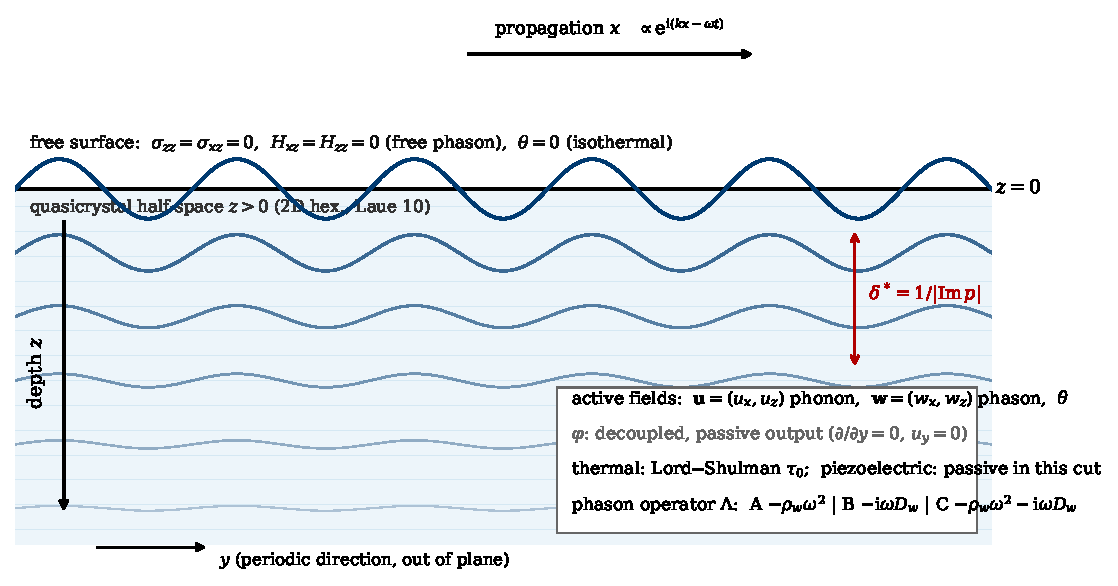
\includegraphics[width=0.98\textwidth]{fig1.pdf}
\caption{Configuration-I schematic: quasicrystal half-space $z>0$ with free surface $z=0$ and the baseline boundary conditions stated at the surface; the sagittal surface wave $\propto\mathrm{e}^{\mathrm{i}(kx-\om t)}$ is drawn at successive depths to indicate exponential localisation with penetration depth $\delta^*=1/|\mathrm{Im}\,p|$ (double arrow); coordinate triad $(x,y,z)$ with $y$ the periodic direction; the field box lists the active fields $(u_x,u_z,w_x,w_z,\tht)$, the passive decoupled potential $\varphi$, the Lord--Shulman time $\tau_0$ (piezoelectricity passive in this cut), and the three phason operators $\Lambda_{A,B,C}$. Conceptual schematic, not a computed result.}
\label{fig:fig1}
\end{figure}

\subsection{Constitutive structure of the 2D hexagonal quasicrystal}

For Laue class~10 (point group 6/mmm) the independent constants number $N_C=5$, $N_K=4$, $N_R=4$ \cite{yang2014,ding2000}. In Configuration~I the plane constitutive equations are
\begin{align}
\sig_{xx}&=C_{11}\e_{xx}+C_{12}\e_{zz}+R_1 w_{x,x}+R_2 w_{z,z}-\beta_1\tht, \label{eq:sxx}\\
\sig_{zz}&=C_{12}\e_{xx}+C_{11}\e_{zz}+R_2 w_{x,x}+R_1 w_{z,z}-\beta_1\tht, \label{eq:szz}\\
\sig_{xz}&=C_{66}\big(\partial_z u_x+\partial_x u_z\big)+R_6\big(\partial_z w_x+\partial_x w_z\big), \label{eq:sxz}
\end{align}
for the phonon stresses, and
\begin{align}
H_{xx}&=R_1\e_{xx}+R_2\e_{zz}+K_1 w_{x,x}+K_2 w_{z,z}, \label{eq:hxx}\\
H_{zz}&=R_2\e_{xx}+R_1\e_{zz}+K_2 w_{x,x}+K_1 w_{z,z}, \label{eq:hzz}\\
H_{xz}&=R_6\big(\partial_z u_x+\partial_x u_z\big)+K_3\,\partial_z w_x+K_6\,\partial_x w_z, \label{eq:hxz}\\
H_{zx}&=R_6\big(\partial_z u_x+\partial_x u_z\big)+K_6\,\partial_z w_x+K_3\,\partial_x w_z, \label{eq:hzx}
\end{align}
for the phason pseudo-stresses. The hexagonal symmetry relations used throughout \cite{yang2014,yang1994prb} are
\begin{equation}
C_{66}=\tfrac12\,(C_{11}-C_{12}),\qquad K_6=K_1-K_2-K_3,\qquad R_6=\tfrac12\,(R_1-R_2). \label{eq:symrels}
\end{equation}
The phason stress is \emph{not symmetric}: $H_{xz}\neq H_{zx}$ unless $K_3=K_6$. This asymmetry is a genuine feature of the 2D hexagonal constitutive structure \eqref{eq:hxz}--\eqref{eq:hzx} (it reflects the fact that the phason pseudo-stress is the conjugate of a displacement \emph{gradient}, not of a symmetric strain); it is preserved exactly in the matrix formulation (Section~3) and must not be symmetrised; symmetrising it would silently alter the sagittal problem.

\subsection{Piezoelectric and thermal coupling}

The piezoelectric constants of the studied class \cite{wang2021,agiasofitou2023} couple the active sagittal fields, in this configuration, only to the passive out-of-plane electric displacement; the electric potential therefore does not appear in the active system (Section~2.1). Thermal coupling enters the phonon stresses through $-\beta_1\tht$ and the heat conduction through $k_{11}$.

\subsection{Phason dynamic models A, B, C}

The phason balance law $\partial_x H_{xx}+\partial_z H_{xz}=\mathcal{L}[w]$ is studied with three dynamic operators $\mathcal{L}$:
\begin{itemize}
\item \textbf{Model A (inertial):} $\rw\,\ddot w=\mathrm{div}\,H$ --- phasons treated as an inertia-carrying field;
\item \textbf{Model B (diffusive):} $\Dw\,\dot w=\mathrm{div}\,H$ --- hydrodynamic dissipative relaxation, $\Dw$ the phason friction;
\item \textbf{Model C (telegraph-type):} $\rw\,\ddot w+\Dw\,\dot w=\mathrm{div}\,H$ --- the wave-telegraph interpolation \cite{agiasofitou2014}.
\end{itemize}
In the harmonic regime these correspond to the phason operators $\Lambda_A=-\rw\om^2$, $\Lambda_B=-\mathrm{i}\om\Dw$, $\Lambda_C=-\rw\om^2-\mathrm{i}\om\Dw$. The phonon momentum balance is $\mathrm{div}\,\sig=\rho\,\ddot u$ in all three models. This three-class taxonomy is not introduced here: it is the wave-telegraph unification of Agiasofitou and Lazar \cite{agiasofitou2014}, in which the elastodynamic wave-type model (attributed there to Ding et al., 1993) and the elasto-hydrodynamic (diffusive) model \cite{lubensky1985} are recovered as asymptotic cases of the telegraph model for extreme values of the phason friction. The present contribution is the surface-wave boundary-value problem built on this taxonomy for the 2D hexagonal class. Model C contains A as the limit $\Dw\to0$ and B as the limit $\rw\to0$; both limits are verified numerically in Section~5.3. Table~\ref{tab:models} summarises the three models.

\begin{table}[t]
\centering
\caption{The three phason dynamic models studied: balance law, harmonic phason operator, degree of $\det M$ in $\om$, limiting relation within model C, and the surface branch found at baseline parameters (Section~6.1).}
\label{tab:models}
\small
\begin{tabular}{@{}lllll@{}}
\toprule
Model & Phason balance law & $\Lambda$ & $\deg_\om\det M$ & Baseline surface branch \\
\midrule
A (inertial) & $\rw\ddot w=\mathrm{div}\,H$ & $-\rw\om^2$ & 10 & phason-dominated, $V^*\approx0.311$ \\
B (diffusive) & $\Dw\dot w=\mathrm{div}\,H$ & $-\mathrm{i}\om\Dw$ & 8 & phonon--Rayleigh, $V^*\approx0.466$ \\
C (telegraph) & $\rw\ddot w+\Dw\dot w=\mathrm{div}\,H$ & $-\rw\om^2-\mathrm{i}\om\Dw$ & 10 & phonon--Rayleigh at baseline \\
\bottomrule
\end{tabular}
\end{table}

\subsection{Lord--Shulman thermoelasticity}

Heat conduction obeys the Lord--Shulman law with a single relaxation time $\tau_0$ \cite{lord1967}:
\begin{equation}
k_{11}\big(\partial_{xx}\tht+\partial_{zz}\tht\big)=\rho c_e\big(\dot\tht+\tau_0\ddot\tht\big)+T_0\beta_1\Big[\big(\dot\e_{xx}+\dot\e_{zz}\big)+\tau_0\big(\ddot\e_{xx}+\ddot\e_{zz}\big)\Big]. \label{eq:LS}
\end{equation}
The nondimensional role of $c_e$ is fixed by the thermal-row normalisation ($c_e^*\equiv1$; the dimensional value is a declared surrogate, Section~4). Two documented modelling assumptions accompany this transcription. First, the phason strain does not enter the heat equation: in the 2D hexagonal constitutive framework \cite{yang2014,wang2021,li2024ijhmt} the temperature couples to the phonon stresses $\sig_{ij}$ but not to the phason pseudo-stresses $H_{ij}$, and the entropy side of the Lord--Shulman energy balance is inherited unchanged --- an assumption of the adopted literature framework, not a derived result. Second, in the limit $\tau_0\to0$ equation~\eqref{eq:LS} reduces to classical coupled thermoelasticity.

\section{Surface-wave formulation}

\subsection{Harmonic plane-wave ansatz}

All fields take the form $\mathrm{exp}[\mathrm{i}(kx+pz-\om t)]$ with real wavenumber $k>0$, complex depth wavenumber $p$, and real frequency $\om>0$. For the half-space $z>0$ the decay condition as $z\to+\infty$ is
\begin{equation}
\mathrm{Im}\,p>0. \label{eq:decay}
\end{equation}
Roots that are nearly real ($|\mathrm{Im}\,p|$ below the admissibility tolerance) are excluded \emph{and flagged} --- never silently reclassified as admissible.

\subsection{Matrix polynomial}

Substitution into the field equations yields the $5\times5$ matrix pencil in the state vector $a=(u_x,u_z,w_x,w_z,\tht)$:
\begin{equation}
M(\om,k,p)\,a=0,\qquad M=A_0+pA_1+p^2A_2. \label{eq:Mpoly}
\end{equation}
The entries follow uniquely from Section~2; in particular the coupling entries that carry the phason-stress asymmetry satisfy the identity
\begin{equation}
A_1(3,4)=A_1(4,3)=-(K_2+K_6)\,k \label{eq:A1ident}
\end{equation}
(indices 1-based). Verified structural properties (symbolic computation, Section~5.2): $\det M$ has degree 10 in $p$ for all three models; degree 10, 8, 10 in $\om$ for models A, B, C respectively; the static determinant factorises as
\begin{equation}
\det M(\om=0)=c\,(k^2+p^2)^5,\qquad c=\frac{410478057}{25600000000000}\ \ \text{(nondimensional)}, \label{eq:statfact}
\end{equation}
and
\begin{equation}
\det(A_2)=\big(C_{11}K_1-R_1^2\big)\big(C_{66}K_3-R_6^2\big)\,k_{11}\,k^4>0, \label{eq:detA2}
\end{equation}
so the ten depth roots are generically non-degenerate.

\subsection{Decaying roots}

For each $(\om,k)$ the ten roots $p_j$ are computed in closed form from the quadratic-in-$p^2$ block structure (depth-root computation with Newton polishing and per-root residual flags) and the five admissible roots with $\mathrm{Im}\,p_j>0$ are retained. Grazing roots (nearly real) are counted separately and flagged. At every reported production branch point the root count was $n_{\mathrm{ad}}=5$, $n_{\mathrm{grazing}}=0$ (Section~5.2, Fig.~\ref{fig:fig8}).

\subsection{Surface boundary conditions}

At $z=0$ the half-space carries the outward normal $n=-e_z$. The baseline (free-surface) conditions are
\begin{equation}
\sig_{zz}=0,\qquad \sig_{xz}=0,\qquad H_{xz}=0,\qquad H_{zz}=0, \label{eq:BCmech}
\end{equation}
supplemented by one thermal condition: isothermal ($\tht=0$) for the production baseline; the insulated alternative ($\partial_z\tht=0$) is implemented but not swept in the production studies. The clamped-phason variant replaces the two phason-traction rows by $w_x=0$, $w_z=0$. The two phason boundary options constrain physically different things: the free condition $H_{xz}=H_{zz}=0$ leaves the surface value of the phason field \emph{undetermined} --- the quasiperiodic structure may re-arrange at the free surface at no phason-stress cost --- whereas the clamped condition $w_x=w_z=0$ pins the quasiperiodic structure at the surface and forces the phason field to adjust in a boundary layer of thickness $\delta^*$ into the material. The taxonomy of these boundary conditions (prescribed traction versus prescribed displacement for each of the phonon, phason, and thermal fields) follows \cite{fan2011,ding2000}. A phason-traction-free surface is not merely a convenient idealisation: it is the condition used for the free surface of a 2D hexagonal quasicrystal half-space in \cite{wang2015}, where the phonon traction and both phason tractions vanish. The 1D hexagonal variant in which only $H_{zz}$ is released (e.g.\ \cite{zhang2023cryst}) is not transferred to the 2D setting, where the phason field carries two independent components. The prescribed normal load follows the convention $t_z=-\sig_{zz}=P_0$, i.e.\ $\sig_{zz}=-P_0$; the eigenproblem uses $P_0=0$. In every case there are five boundary conditions for the five admissible depth roots, so the half-space problem is determined for each of the three models.

\subsection{Surface determinant and singular-value criterion}

Assembling the five admissible partial waves into the $5\times5$ boundary matrix $B(\om,k)$ (rows in the order of Section~3.4), a surface wave exists when $B$ is singular:
\begin{equation}
\det B(\om,k)=0. \label{eq:secular}
\end{equation}
The numerical indicator is
\begin{equation}
r(\om,k)=\frac{\sigma_{\min}\big(B(\om,k)\big)}{\lVert B(\om,k)\rVert}, \label{eq:rind}
\end{equation}
minimised over $k$ at fixed $\om$. The normalisation by $\lVert B\rVert$ is recorded rather than assumed to be innocuous: $r$ is \emph{not} invariant under arbitrary row rescalings, and no such invariance is claimed anywhere in this work; the system is solved in nondimensional variables, and the conditioning $\kappa(B)$ (up to $\sim5\times10^8$ at some points) and the per-point residual floors ($10^{-11}$--$5.6\times10^{-6}$) are stored with every result.

\subsection{Numerical root tracking}

The surface-wave speed is reported as $V^*=\Om/k^*$ (nondimensional phase speed; Section~4). Branches are tracked by continuation with (i)~a global scan with sub-scans at the bulk-grazing wavenumbers $k_g=\Om/v_c$, $v_c\in\{\sqrt{C_{11}^*},\sqrt{C_{66}^*},\sqrt{K_3^*}\}$; (ii)~a continuation-preferred selection with a staleness guard; (iii)~rejection of quasi-static degenerate minima ($V^*<0.15$, whereas every physical branch of this system has $V^*\ge0.29$) --- points lacking a physical candidate are reported as degenerate-only and never substituted; (iv)~branch-identity-verified seeds for model-limit sweeps (the seed must match the corresponding limit model's tracked branch; Section~5.3); and (v)~a branch-jump diagnostic that fails the sweep on any unexplained change of $V^*$ exceeding 5\% between neighbours. An independent two-path consistency check (the production $\om\to k^*$ route versus the alternate $k^*\to\om$ route) precedes any production sweep.

\section{Nondimensionalization and parameters}

Lengths are scaled by $k_0^{-1}$ with the declared reference scale $k_0=2\pi\times10^{6}\,\mathrm{m^{-1}}$ (reference wavelength $1\,\mu$m; $k_0$ is a scale, never a working wavenumber --- the working wavenumber is the solved $k$), velocities by $v_0=\sqrt{C_{11}/\rho}$, frequencies by $\om_0=v_0k_0$, displacements by $U_0=\beta_1T_0/(C_{11}k_0)$ with $W_0=U_0$, temperature by $T_0$, and stresses by $C_{11}$. Starred symbols denote nondimensional quantities; $\Om=\om/\om_0$, $k^*=k/k_0$, $V^*=\Om/k^*$, $p^*=p/k_0$.

The computed scales for the accepted parameter set (Table~\ref{tab:params}) are
\begin{equation}
v_0=6917.1446\ \mathrm{m/s},\qquad \om_0=4.34617\times10^{10}\ \mathrm{rad/s},\qquad U_0=W_0=4.2636\times10^{-10}\ \mathrm{m}. \label{eq:scales}
\end{equation}
The nondimensional baseline is
\begin{align}
&C_{11}^*=1,\ C_{12}^*=0.5,\ C_{66}^*=0.25;\quad K_1^*=0.25,\ K_2^*=K_3^*=0.1,\ K_6^*=0.05; \nonumber\\
&R_1^*=0.05,\ R_2^*=0.025,\ R_6^*=0.0125;\quad \rho^*=\rw^*=1,\ \beta_1^*=1,\ c_e^*=1; \nonumber\\
&k_{11}^*=2.6077\times10^{-3},\quad \tau_0^*=4.3462\times10^{-3},\quad T_0\beta_1^*=2.3047\times10^{-3},\quad D_w^*=11467.5. \label{eq:starred}
\end{align}
Table~\ref{tab:nondim} collects the controlling nondimensional groups and the ranges actually swept in this work. The friction value defines the phason crossover frequency $\om_c=\Dw/\rw$ (from model C's dynamic operator), i.e.
\begin{equation}
\Om_c=D_w^*/\rw^*=11467.5,\qquad \om_c\approx4.984\times10^{14}\ \mathrm{rad/s},\qquad f_c=\om_c/2\pi\approx79.32\ \mathrm{THz}, \label{eq:omegac}
\end{equation}
and the telegraph relaxation scale $\tau_{\mathrm{tel}}^*=1.744\times10^{-4}$, i.e.\ $\tau_{\mathrm{tel}}=2/\om_c\approx4.013\times10^{-15}$~s. $\Om_c$ appears in the results only as a reference line (Section~6.2); it is not presented as a validated transition.

\begin{table}[t]
\centering
\caption{Dimensional parameter set (provenance as recorded; the set is composite and partly surrogate --- see Section~7.9).}
\label{tab:params}
\small
\begin{tabular}{@{}p{2.4cm}p{7.6cm}p{4.6cm}@{}}
\toprule
Group & Values & Status \\
\midrule
Phonon elastic & $C_{11}=200$, $C_{12}=100$, $C_{13}=100$, $C_{33}=150$, $C_{44}=50$, $C_{66}=50$~GPa & composite literature table \cite{wang2021,li2017}; $C_{66}=(C_{11}-C_{12})/2$ \\
Phason elastic & $K_1=50$, $K_2=20$, $K_3=20$, $K_4=20$, $K_6=10$~GPa & same table; $K_6$ derived \\
Coupling & $R_1=10$, $R_2=5$, $R_3=5$, $R_4=3$, $R_6=2.5$~GPa & same table; $R_6$ derived \\
Piezoelectric & $e_{31}=-0.160$, $e_{33}=-0.347$, $e_{15}=-0.138$; $e'_{31}=-0.350$, $e'_{15}=-0.160$~C/m$^2$ & same table (passive in this configuration) \\
Dielectric & $\xi_{11}=82.6$, $\xi_{33}=90.3$~pF/m & same table (passive in this configuration) \\
Thermal & $\beta_1=1.798$, $\beta_3=1.383$~MPa/K; $k_{11}=k_{33}=6$~W/(m\,K); $T_0=298$~K; $c_e=500$~J/(kg\,K) & $k_{11}$: declared choice 6; \cite{li2017} reports 5.3 --- discrepancy genuine and unresolved (see text). $c_e$: surrogate, from $c_p\approx25$~J/(mol\,K) \cite{hosseini2019} with declared $M\approx50$~g/mol \\
Inertia & $\rho=4180$~kg/m$^3$; $\rw=\rho$ & surrogate (decagonal-QC data \cite{hosseini2019,chellappan2015}); $\rw=\rho$ declared --- no independent phason mass density in the literature \\
Phason friction & $\Dw=2.0833\times10^{18}$, from $\Dw=1/C_w$, $C_w=4.8\times10^{-19}\,\mathrm{m^3\,s/kg}$ \cite{chellappan2015} & literature-derived \\
Relaxation & $\tau_0$ swept $10^{-13}$--$10^{-11}$~s in design; production study uses $\tau_0^*$ values & declared computational parameter \\
\bottomrule
\end{tabular}
\end{table}

\begin{table}[t]
\centering
\caption{Controlling nondimensional groups and swept ranges (baseline values from \eqref{eq:starred}).}
\label{tab:nondim}
\small
\begin{tabular}{@{}llp{6.05cm}@{}}
\toprule
Group & Baseline & Swept range (where applicable) \\
\midrule
Frequency $\Om^*$ & --- & $10^{-3}$--$10^{3}$ (121 pts, Studies 1, 3); $10^{-3}$--$10^{2}$ (61 pts, Study 2) \\
Phason friction $D_w^*$ & $11467.5$ & $10^{-2}$--$10^{4}$ (61 values, Study~2) \\
Relaxation time $\tau_0^*$ & $4.3462\times10^{-3}$ & $\{10^{-5},10^{-4},4.3462\times10^{-3},10^{-2},10^{-1}\}$ (Study~3) \\
Phason crossover $\Om_c=D_w^*/\rw^*$ & $11467.5$ & reference line only (no transition claimed) \\
Thermoelastic coupling $T_0\beta_1^*$ & $2.3047\times10^{-3}$ & fixed (baseline) \\
Resolution floor $\e_\Delta$ (absolute $V$) & $1.13\times10^{-8}$ & benchmarked, fixed \\
\bottomrule
\end{tabular}
\end{table}

The parameter set is a \emph{composite/surrogate} set: no single fully characterised 2D hexagonal quasicrystal specimen provides all of these constants experimentally. All conclusions are therefore statements about the model with these parameters, not about a specific material. The thermal conductivity illustrates the point: the adopted $k_{11}=6$~W/(m\,K) differs from the $5.3$~W/(m\,K) tabulated in \cite{li2017}; the discrepancy is genuine, unresolved in the source literature, and declared --- $k_{11}$ enters only the thermal row of the formulation.

\section{Verification and benchmarks}

All verifications were executed as automated steps on the final implementation, before and alongside the production studies; the complete records ship with the reproducibility package.

\subsection{Classical elastic and Rayleigh benchmark}

With phason and thermal fields frozen out, the decoupled elastic limits are exact: $v_P/v_0=1$ and $v_S/v_0=1/2$ to machine precision (nondimensionally, $\sqrt{C_{11}^*/\rho^*}=1$, $\sqrt{C_{66}^*/\rho^*}=1/2$). For the classical Poisson ratio $\nu=1/3$ implied by $C_{12}^*=0.5$, the decoupled Rayleigh ratio computed by the production machinery is
\begin{equation}
v_R/v_S=0.932525905921\quad\text{versus the analytic}\quad 0.932525905931, \label{eq:rayleigh}
\end{equation}
a relative discrepancy of $1.1\times10^{-11}$ (Fig.~\ref{fig:fig2}). In the fully coupled quasi-static limit with a free phason surface, the models B and C give $V^*/v_S=0.9326028$ (e.g.\ $0.93260276$ at $\Om=10^{-5}$), i.e.\ $+7.7\times10^{-5}$ above the decoupled analytic Rayleigh value --- the phason surface compliance effect; model A gives $V^*/v_S=0.62145378$ at the same limit, its distinct phason-dominated branch.


\begin{figure}[htbp]
\centering
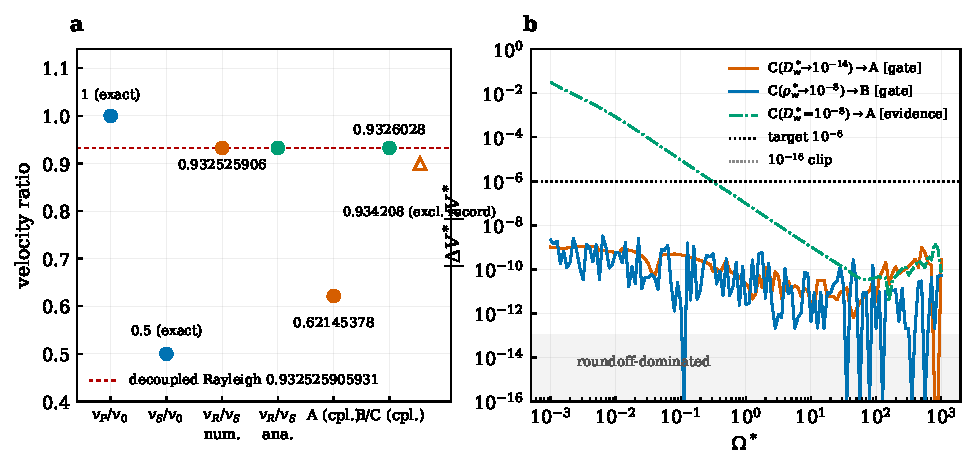
\includegraphics[width=0.98\textwidth]{fig2.pdf}
\caption{Verification. (a)~Classical-limit benchmarks: nondimensional bulk speeds $v_P/v_0=1$ and $v_S/v_0=0.5$ (exact), the decoupled Rayleigh ratio computed by the production machinery ($0.932525906$) against the analytic value $0.932525905931$ (dashed line; relative error $1.1\times10^{-11}$), the coupled quasi-static free-phason ratios $0.62145378$ (model A) and $0.9326028$ (models B/C), and the excluded exploratory coarse-scan record $0.934208$ (open marker; Section~5.1). (b)~Model-limit reproduction on the full grid: C($D_w^*\to10^{-14}$)$\to$A and C($\rw^*\to10^{-8}$)$\to$B gates ($121/121$ within $10^{-6}$; maxima $1.11\times10^{-9}$, $3.27\times10^{-9}$) and the frozen $10^{-8}$ evidence curve (dash-dot) leaving the target below $\Om^*\approx0.32$ with the non-uniform singular-limit envelope $\sim\Om_c/\Om^*$; the shaded band marks the roundoff-dominated region at the $10^{-16}$ clip, and the deep dips of the gate curves into that band are double-precision cancellation, not solver failure.}
\label{fig:fig2}
\end{figure}

What Fig.~\ref{fig:fig2} establishes, and what it rules out: the production machinery reproduces the classical theory exactly wherever classical theory applies, so every deviation reported later is attributable to the quasicrystal couplings rather than to the formulation or the root tracking. The spread between the three model markers in the coupled column is the first visible signature of the central result of this paper: with a free phason surface, the inertial phason (model A) does not follow the phonon--Rayleigh branch at all.

\subsection{Structural and symbolic verification}

Symbolic verification (exact rational arithmetic): $\deg_p\det M=10$ for models A, B, C; $\deg_\om\det M=10,8,10$ for A, B, C (model B loses the phason-inertia terms, reducing the frequency degree by two); $\det M(\om=0)=\frac{410478057}{25600000000000}(k^2+p^2)^5$ for all three models; $\det A_2>0$ with the factorisation \eqref{eq:detA2}. The nondimensional arithmetic of Section~4 is reproduced exactly ($c_e^*\equiv1$ by construction). In the production diagnostics, every reported branch point carries five admissible decaying roots and zero grazing roots ($n_{\mathrm{ad}}=5$, $n_{\mathrm{grazing}}=0$ at $\Om=0.1,10,1000$ for all three models; Fig.~\ref{fig:fig8}), with per-point branch residuals $9.7\times10^{-9}$--$3.2\times10^{-5}$ recorded.

\begin{figure}[htbp]
\centering
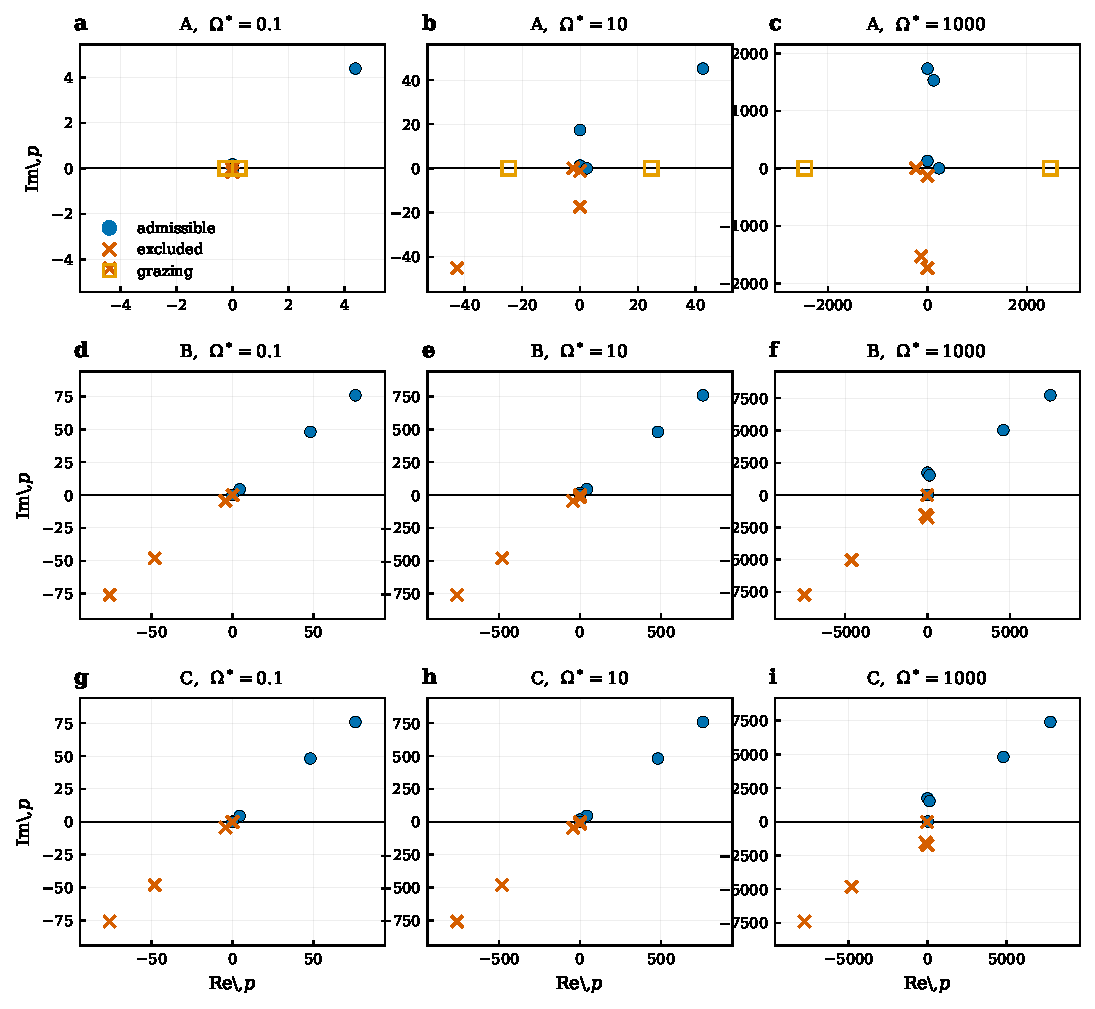
\includegraphics[width=0.98\textwidth]{fig8.pdf}
\caption{Depth-root structure of the pencil $M(\Om^*,k^*,p)$ at $k^*=2\Om^*$; rows: models A, B, C; columns: $\Om^*=0.1,10,1000$; panels (a)--(i). Circles: admissible decaying roots ($\mathrm{Im}\,p>0$; five per panel, so the $5\times5$ boundary problem is determined everywhere); crosses: excluded roots; open squares: grazing (nearly real) roots, shown in the model-A panels where they accompany the documented near-grazing degeneracy ($V^*<\sqrt{K_3^*}$). Admissible residuals $\le6.0\times10^{-17}$; excluded roots carry no accepted residual by construction; the mirror symmetry about $\mathrm{Im}\,p=0$ reflects the real-coefficient depth problem.}
\label{fig:fig8}
\end{figure}

Fig.~\ref{fig:fig8} answers the structural question behind every number reported in this paper: at all three decades of frequency and for all three models the root set splits cleanly into five decaying and five excluded roots, with no root crossing the real axis at the reported branch points (grazing roots appear only in the model-A panels, adjacent to the degenerate region, and are never counted as admissible). What does \emph{not} change across the panels --- the count $n_{\mathrm{ad}}=5$ --- is what licenses the uniform $5\times5$ surface formulation; what does change is the geometric arrangement of the admissible cluster, reflecting the different balance of phason inertia and friction encoded in each model.

\subsection{Model-limit verification (C $\to$ A and C $\to$ B)}

On the full Study-1 grid ($\Om=10^{-3}$--$10^{3}$, 121 logarithmic points; Fig.~\ref{fig:fig2}):
\begin{itemize}
\item \textbf{C($D_w^*\to10^{-14}\times$baseline) $\to$ A:} $\max|\Delta V|/V=1.11\times10^{-9}$, all 121/121 points within the frozen $10^{-6}$ target.
\item \textbf{C($\rw^*\to10^{-8}\times$baseline) $\to$ B:} $\max|\Delta V|/V=3.27\times10^{-9}$, 121/121.
\item \textbf{Evidence curve C($D_w^*=10^{-8}\times$baseline) $\to$ A} (frozen design perturbation, retained but not gated): meets $10^{-6}$ for $\Om\ge0.3162$ (71/121 points). Below that crossover the deviation grows smoothly with the singular-limit envelope $\sim\Om_c/\Om$ (here $\Om_c=1.1467\times10^{-4}$), reaching $3.1\times10^{-2}$ at $\Om=10^{-3}$. This is genuine perturbation physics --- the $\Dw\to0$ limit is not uniform in $\Om$ --- not a numerical failure.
\end{itemize}
The limit sweeps are tracked downward from the top of the grid with \emph{branch-identity-verified seeds}: at the seed frequency the continuation start must be the local minimum of $r$ that connects continuously (in model space) to the corresponding limit model's tracked branch, accepted within a $10^{-2}$ relative branch-match tolerance, otherwise the sweep fails outright. This protocol was introduced after a wrong-branch seeding artefact was identified at $\Om=10^3$ (the seedless global minimum can sit on the phonon branch, $V^*\approx0.467$, while the intended phason branch is a narrow near-grazing minimum at $V^*\approx0.3107$); with the fix, the seed is verified at $V^*=0.31072662$ (deviation $7.6\times10^{-11}$ from A), the maximum neighbour-to-neighbour relative change along the whole evidence curve is $5.4\times10^{-3}$, and a branch-jump diagnostic reports no discontinuities on any of the six tracked sweeps. The isolated dips of the gate curves into the shaded $10^{-16}$ band of Fig.~\ref{fig:fig2}(b) are double-precision cancellation between nearly equal speeds (the limit is reproduced to $\sim10^{-9}$), classified as numerical roundoff and retained without smoothing.

A two-path consistency check (production $\om\to k^*$ route versus the independent $k^*\to\om$ route) passes 15/15 anchors with worst relative difference $1.04\times10^{-9}\le10^{-8}$ before any physics sweep.


Fig.~\ref{fig:fig2} is the numerical certificate that model C is a genuine interpolation rather than a third unrelated theory: as the friction is removed C reproduces the inertial model, as the phason inertia is removed it reproduces the diffusive model, over the whole grid and to parts per billion. The dashed evidence curve adds the physically instructive failure mode of the opposite kind: at any \emph{finite} residual friction the C$\to$A limit is non-uniform in frequency, because the ratio $\Om/\Om_c$ --- the competition parameter of Section~7.4 --- grows without bound as $\Om\to0$ at fixed small $\Dw$. The curve is therefore kept in the paper: it documents exactly where the formal limit must be used with care, and it is the reason the production statements of Section~6 always carry their $\Om$ ranges.

\subsection{Boundary-condition and thermal checks}

The boundary-matrix construction is exercised by the production boundary-condition study (Section~6.6): model C clamped-versus-free differs by at most $8.1\times10^{-6}$ relative in $V^*$, a small but resolvable effect; model A shows \emph{no comparable clamped branch at all} (Section~6.6) --- recorded as a structural finding, not plotted as a difference. The isothermal/insulated thermal boundary options are implemented; a production isothermal-versus-insulated sweep is not part of the accepted studies, and no thermal-boundary-condition effect size is claimed (not established by the present study). Thermal relaxation is instead probed through the $\tau_0^*$ sweep (Section~6.5).

\section{Results}

Numerical resolution (benchmark, refinement-based, recorded in the reproducibility package): branch-position uncertainty $u_V\le1.13\times10^{-9}$; the model-difference threshold is fixed as $\e_\Delta=10\max u_V=1.13\times10^{-8}$ \emph{in absolute $V$ units}. Relative differences such as $\Delta_{BC}=|V_B-V_C|/V_C$ are compared against the corresponding relative floor $\e_\Delta/V_C^*\approx2.42\times10^{-8}$; this is mathematically identical to the absolute statement $|V_B-V_C|<\e_\Delta$. Differences below the floor are reported as ``indistinguishable within numerical resolution'' --- never as exactly zero, never as significant.

\subsection{Baseline A/B/C surface-wave response (RQ1)}

The first question is whether the three phason dynamic classes even support the same surface wave. Over $\Om=10^{-3}$--$10^{3}$ (121 points, free phason, isothermal; Figs.~\ref{fig:fig3}--\ref{fig:fig4}):
\begin{itemize}
\item \textbf{Model A} tracks a single phason-dominated branch, $V^*_A\approx0.31073$ across the whole range ($0.31072689$ at $\Om=10^{-3}$ to $0.31072662$ at $\Om=10^{3}$), with phason amplitude participation $P_w\approx0.991$ and penetration depth $\delta^*=19.9$ at $\Om=0.1$ shrinking as $1/\Om$ (Fig.~\ref{fig:fig11}).
\item \textbf{Models B and C} track the phonon--Rayleigh branch, $V^*\approx0.46630\to0.46626$ over the grid, with $P_w$ between $1.7\times10^{-13}$ ($\Om=0.1$) and $1.8\times10^{-5}$ ($\Om=10^{3}$) --- phonon-dominated at every reported point --- and $\delta^*\approx12.9\to1.3\times10^{-3}$ (Fig.~\ref{fig:fig11}).
\item The B--C relative difference satisfies $\Delta_{BC}\le9.5\times10^{-6}$ (maximum at $\Om=10^{3}$), and \textbf{95 of 121 grid points lie below the resolution floor} $\e_\Delta/V_C^*\approx2.42\times10^{-8}$ (equivalently $|V_B-V_C|<\e_\Delta$).\footnote{For completeness: comparing $\Delta_{BC}$ directly against the numeric value $1.13\times10^{-8}$ treated as a dimensionless threshold --- a comparison that omits the $1/V_C^*$ conversion and is dimensionally inconsistent --- would give 91/121; no conclusion depends on this reading.} B and C are therefore indistinguishable at baseline over most of the swept range within numerical resolution.
\item The A--C difference is large, $\Delta_{AC}\approx0.334$: model A is separated from B/C by a \emph{different branch} (phason-dominated versus phonon--Rayleigh), not by a small perturbation effect.
\end{itemize}

\begin{figure}[htbp]
\centering
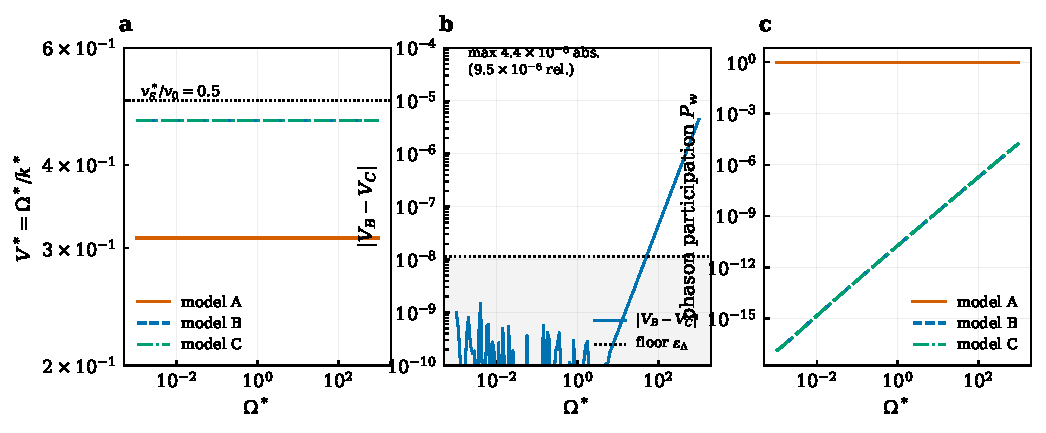
\includegraphics[width=0.98\textwidth]{fig3.pdf}
\caption{Baseline surface response (free phason, isothermal). (a)~$V^*=\Om^*/k^*$ versus $\Om^*$ for models A (solid), B (dashed), C (dash-dot) with the bulk-shear reference $v_S^*/v_0=0.5$: model A on the phason-dominated branch ($V^*\approx0.311$), B and C on the phonon--Rayleigh branch ($V^*\approx0.466$). (b)~Absolute B--C separation $|V_B-V_C|$ against the absolute resolution floor $\e_\Delta=1.13\times10^{-8}$ (shaded sub-floor region: indistinguishable); the separation grows to $4.4\times10^{-6}$ absolute ($9.5\times10^{-6}$ relative) at the top of the band. (c)~Phason participation $P_w$: $\approx0.99$ for A (phason-carried mode) versus $\le1.8\times10^{-5}$ for B/C (phonon-carried modes) --- the mode-character counterpart of the branch split in (a).}
\label{fig:fig3}
\end{figure}

Fig.~\ref{fig:fig3}(a) shows two flat-to-slightly-decreasing curves that never approach each other. What is plotted is the phase speed of the \emph{same boundary-value problem} solved under three phason laws; what changes between the models is which local minimum of $r$ the branch tracker follows, and that choice is physical, not numerical: the model-A minimum is a narrow phason resonance (Section~6.3), while the B/C minimum is the classical Rayleigh minimum modified by phason compliance (Fig.~\ref{fig:fig2}). Both branches lie below the bulk-shear line $v_S^*/v_0=0.5$, as a surface branch must. Panel (b) zooms into the B--C pair in absolute units: the separation is invisible on the scale of (a), stays below the absolute floor $\e_\Delta$ over most of the band, and only lifts to $4.4\times10^{-6}$ at the top --- the visual form of ``indistinguishable at baseline''. Panel (c) states the mechanism: $P_w\approx0.99$ for A makes its mode a phason-carried wave, whereas $P_w\le1.8\times10^{-5}$ for B/C makes theirs phonon-carried waves dressed by a slaved phason shadow. The near-flatness of $V^*(\Om^*)$ means the reported effects are branch-selection effects at essentially fixed frequency --- dispersion plays no significant role inside the swept band.

\begin{figure}[htbp]
\centering
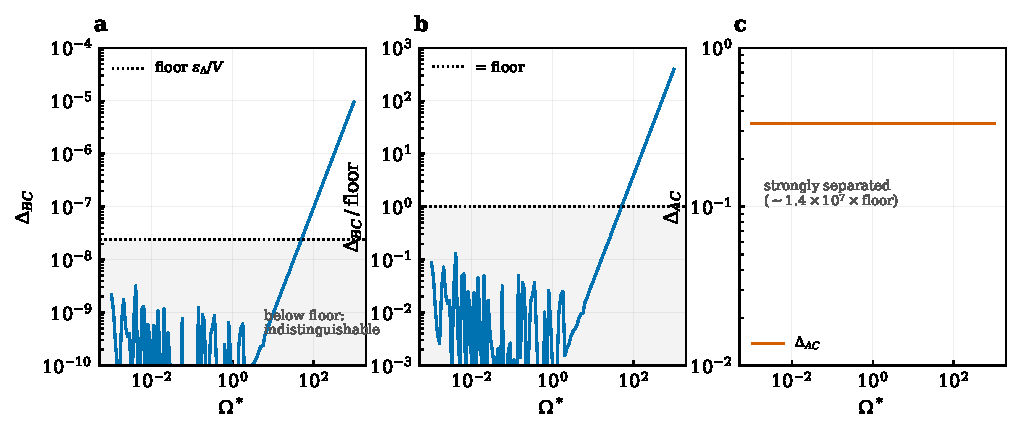
\includegraphics[width=0.98\textwidth]{fig4.pdf}
\caption{Baseline model differences and the resolution logic. (a)~Relative $\Delta_{BC}$ with the relative floor $\e_\Delta/V\approx2.42\times10^{-8}$; the shaded sub-floor region is indistinguishable within numerical resolution (95/121 points). (b)~The same data divided by the floor: values below unity are indistinguishable, values above unity resolvable; the curve crosses unity only above $\Om^*\approx6$. (c)~$\Delta_{AC}\approx0.334$, i.e.\ $\sim1.4\times10^{7}$ times the floor: models A and C differ by branch identity, not by a small perturbation.}
\label{fig:fig4}
\end{figure}

Fig.~\ref{fig:fig4} converts the same result into difference language and makes the resolution logic explicit. The constant $\Delta_{AC}\approx0.334$ is a branch-identity statement, not a parameter-sensitivity statement: it does not shrink at any frequency in the band because the two models are on different modes. The $\Delta_{BC}$ curve, by contrast, wanders about the resolution floor --- at most $9.5\times10^{-6}$ relative, at 95/121 points below $2.42\times10^{-8}$ --- which is the quantitative form of the claim ``diffusive and telegraph phasons are observationally the same surface wave at baseline friction''. Panel (b) makes the resolution logic dimensionless: $\Delta_{BC}$ divided by the floor is below unity (indistinguishable) up to $\Om^*\approx6$ and reaches $\sim4\times10^{2}$ at the top of the band --- resolvable, but still a perturbation. The honest reading of the residual structure above the floor at the top of the band is that the diffusive/telegraph difference \emph{grows} with $\Om$ (as $\Om/\Om_c$ grows, Section~7.4) and would become resolvable at higher $\Om$ or lower $D_w^*$ --- which is exactly what the controlled-friction study of Section~6.4 finds.

Interpretation for RQ1: at the baseline friction $D_w^*=11467.5$ ($\Om_c=11467.5\gg\Om_{\max}=10^3$), the telegraph model C operates deep inside its inertia-suppressed, friction-dominated regime on the whole swept grid, and its surface branch is numerically indistinguishable from the purely diffusive model B. The inertial model A, by contrast, supports a genuinely different --- phason-dominated and slower --- surface branch. The dynamical class of the phason field thus matters qualitatively (A versus B/C) but not, at baseline friction within the swept range, quantitatively between B and C.

\subsection{Phason dynamics and the crossover (RQ2)}

The operator crossover of model C, $|\rw\Om^2|\sim|\Dw\Om|$ at $\Om_c=D_w^*/\rw^*$, is a property of the phason dynamic operator. It must not be confused with an observable crossover in $\Delta_{BC}$: the production data show no resolvable $\Delta_{BC}$ feature at $\Om_c$ for the baseline friction (Section~6.1). The curves $\Om_c(D_w^*)=D_w^*/\rw^*$ are drawn on Figs.~\ref{fig:fig9} \emph{as reference lines only}; the present computations do not establish them as transitions of any observable.

\subsection{Diffusive/inertial/telegraph limits (RQ1, RQ2)}

Section~5.3 established the formal limits C$\to$A ($D_w^*\to10^{-14}$) and C$\to$B ($\rw^*\to10^{-8}$) on the full grid to $\le3.3\times10^{-9}$, with the frozen $10^{-8}$ evidence curve quantifying where the $\Dw\to0$ limit ceases to be uniform ($\Om\lesssim0.316$ at that perturbation; envelope $\sim\Om_c/\Om$). The model-C family therefore genuinely contains both dynamical classes, and which limit is approached at a given frequency is controlled by $\Om/\Om_c$ --- but, per Section~6.1, at the baseline friction this control parameter is small over the entire production range, which is exactly why B and C coincide there.

\subsection{Effect of $D_w^*$ (RQ2)}

If the baseline insensitivity of $\Delta_{BC}$ is caused by large friction, reducing the friction should expose the diffusive/telegraph difference. A $61\times61$ map over $\Om=10^{-3}$--$10^{2}$ and $D_w^*=10^{-2}$--$10^{4}$ (models B and C; all 3721 points resolved and physical, $V_B^*\ge0.4650$, $V_C^*\ge0.4663$; Figs.~\ref{fig:fig5}, \ref{fig:fig9}):
\begin{itemize}
\item $\Delta_{BC}$ (relative) ranges from $0$ to $5.0\times10^{-3}$; 2377/3721 points lie above the per-point relative resolution floor.
\item The \emph{resolvable region slides with $D_w^*$}: at $D_w^*=10^{-2}$--$10^{0}$, $\Delta_{BC}$ (maximum $\approx5.0\times10^{-3}$) exceeds the floor over essentially the whole frequency range (from $\Om\approx10^{-3}$ and $\Om\approx4.6\times10^{-3}$ respectively); at $D_w^*=10^{2}$ only for $\Om\ge0.46$ (maximum $9.9\times10^{-4}$); at $D_w^*=10^{4}$ (baseline scale) $\Delta_{BC}\le1.25\times10^{-7}$ --- indistinguishable except at the very top of the range ($\Om\ge46$).
\end{itemize}

\begin{figure}[htbp]
\centering
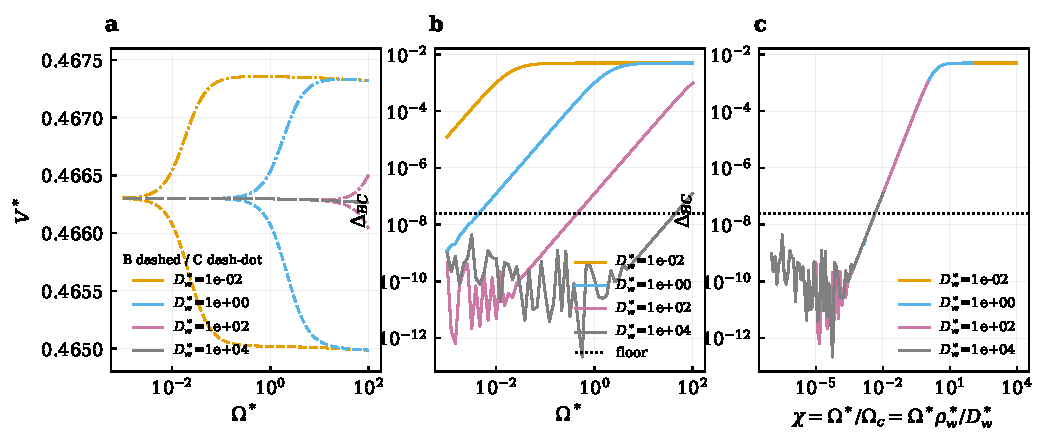
\includegraphics[width=0.98\textwidth]{fig5.pdf}
\caption{Controlled-friction study (Study~2). (a)~$V^*(\Om^*)$ for models B (dashed) and C (dash-dot) at $D_w^*=10^{-2},10^{0},10^{2},10^{4}$ (colours): the relaxation shoulder of the C branch shifts systematically toward higher $\Om^*$ as $D_w^*$ increases, while the B--C offset shrinks. (b)~$\Delta_{BC}(\Om^*)$ at the same frictions with the resolution floor: the resolvable window opens toward lower frequency as $D_w^*$ decreases (maximum $\approx5.0\times10^{-3}$ at $D_w^*=1$; $\le1.25\times10^{-7}$ at $D_w^*=10^{4}$). (c)~The same differences plotted against the competition coordinate $\chi=\Om^*/\Om_c=\Om^*\rw^*/D_w^*$: the four frictions collapse onto a single master curve, showing that $\chi$ organises the diffusive/telegraph separation; the low-$\chi$ scatter at or below the floor is the indistinguishable regime. All curves are raw $61$-point grid slices; no interpolation.}
\label{fig:fig5}
\end{figure}

Fig.~\ref{fig:fig5} displays the mechanism directly. In panel (a) the wave speeds change only marginally: the B/C branch moves by at most $\sim10^{-3}$ across four decades of friction, so the friction does not restructure the surface wave --- it changes \emph{which description} of the phason field the wave sees; the relaxation shoulder of the C branch slides toward higher $\Om^*$ as $D_w^*$ increases. Panel (b) is where the physics of RQ2 lives: the $\Delta_{BC}$ curves are ordered by $D_w^*$ and slide systematically along the frequency axis. The ordering is the signature of the competition parameter $\Om/\Om_c$: for a fixed frequency, lowering $D_w^*$ raises $\Om/\Om_c$, and the telegraph model's inertial term $-\rw\om^2$ becomes comparable to its friction term $-\mathrm{i}\om\Dw$, separating it from the purely diffusive model. Panel (c) sharpens this: plotted against the single coordinate $\chi=\Om^*/\Om_c$, the four friction levels collapse onto one master curve --- the B--C separation is a function of the inertia/friction ratio, not of friction alone. That the largest difference is still only $\approx5\times10^{-3}$ relative --- resolvable, but small --- is itself a result: even at $D_w^*=1$, four decades below baseline, the surface wave remains overwhelmingly a phonon--Rayleigh wave, and the phason dynamics modifies it perturbatively.

\begin{figure}[htbp]
\centering
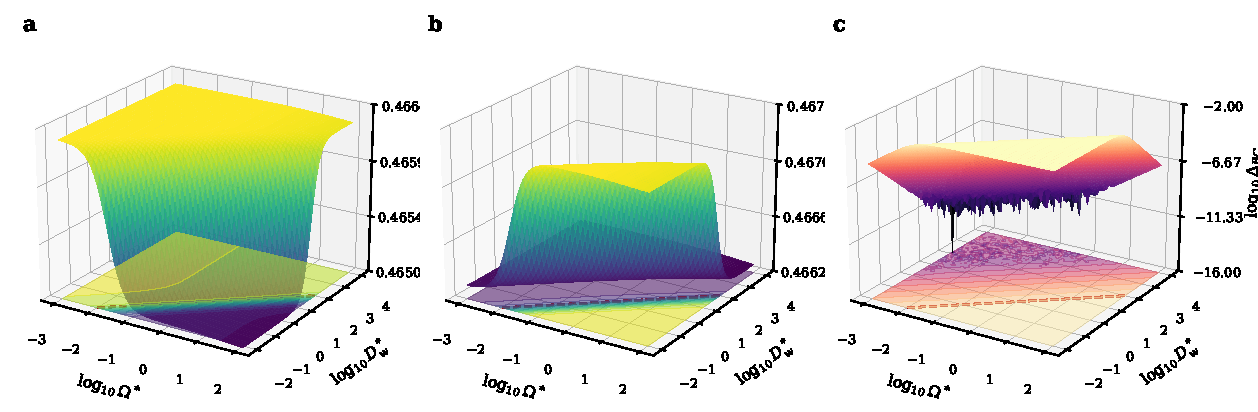
\includegraphics[width=0.98\textwidth]{fig9.pdf}
\caption{Three-dimensional representation of the full Study-2 grid ($61\times61$ computed points; no interpolation; contours projected onto the base plane): (a)~$V_B^*(\Om^*,D_w^*)$ and (b)~$V_C^*(\Om^*,D_w^*)$ surfaces, with $z$-axes spanning exactly the data ranges $[0.4650,0.4664]$ and $[0.4662,0.4674]$ (no vertical exaggeration) --- both surfaces are gently sloped phonon--Rayleigh sheets with the S-shaped relaxation ridge of the C family; (c)~$\log_{10}\Delta_{BC}(\Om^*,D_w^*)$: the resolvable plateau (upper, $\gtrsim-3$) at low $D_w^*$ and the resolution-indistinguishable skirt at the $-16$ clip, where $\Delta_{BC}$ is numerically zero, are separated by a smooth front sliding with $D_w^*$. The dashed base curve is the operator crossover $\Om_c=D_w^*/\rw^*$, drawn as a reference line only --- no observable transition is claimed at it.}
\label{fig:fig9}
\end{figure}

The 3D surfaces of Fig.~\ref{fig:fig9}(a,b) exist to establish what the friction does \emph{not} do: even over four decades of $D_w^*$ and five decades of $\Om^*$, both $V_B^*$ and $V_C^*$ form gently sloped sheets confined to a narrow band below the classical Rayleigh ratio, and the two surfaces are visually identical at the plotted $z$-range (which spans exactly the data, without exaggeration). The surface wave is robust to the phason dynamics class in its speed; the distinguishing information is in the small difference between the sheets, which panel (c) makes explicit.


Fig.~\ref{fig:fig9}(c) is the compact answer to RQ2. Reading the surface against the resolution floor ($\log_{10}\Delta\approx-7.6$), the resolvable region is a plateau--front--skirt structure anchored at low friction: at $D_w^*\le10^{0}$ essentially the whole frequency axis is resolvable, at $D_w^*=10^{2}$ only $\Om^*\gtrsim0.46$, and at the baseline $D_w^*\approx10^{4}$ the surface sits in the noisy skirt at the $-16$ clip, i.e.\ in the region where $\Delta_{BC}$ is numerically zero and B/C are indistinguishable. Two cautions belong to the reading of this figure. First, the front between plateau and skirt is a \emph{resolution boundary}, not a material transition: it is where the model difference crosses the numerical floor, and the floor is a property of the solver, not of the quasicrystal. Second, the dashed $\Om_c$ curve on the base plane runs diagonally; the data show the resolvable plateau opening \emph{before} (to the left of and below) that line, so the surface-wave separability is not organised by the bare operator crossover --- consistent with the branch-perturbation reading of Section~7.4 rather than with a mode-transition reading. No phase transition is claimed at any curve in this figure.

This is the quantitative answer to RQ2: the choice between diffusive and telegraph phason dynamics is observable in the surface wave \emph{only when the friction is low enough (or the frequency high enough) relative to $\rw$}; at the baseline friction the two descriptions are numerically indistinguishable over the swept band, and the paper claims exactly that --- neither a null result nor an amplified difference.

\subsection{Thermal relaxation (RQ3)}

Sweeping $\tau_0^*\in\{10^{-5},10^{-4},4.3462\times10^{-3},10^{-2},10^{-1}\}$ over the Study-1 grid (isothermal surface; Figs.~\ref{fig:fig6}, \ref{fig:fig10}): the maximum relative change of $V^*$ against the $\tau_0^*$-reference is $\max\Delta_T=7.9\times10^{-5}$, attained at the largest relaxation time --- small, but approximately three orders of magnitude above the resolution floor, hence a \emph{weak, resolvable} thermal-relaxation effect. Near the baseline $\tau_0^*=4.3462\times10^{-3}$ the effect is at or below the floor. The honest summary for RQ3: within the swept parameter range the Lord--Shulman relaxation modifies the surface wave weakly; it is not negligible at large $\tau_0^*$, and it is not significant near baseline. A thermal \emph{boundary-condition} comparison (isothermal versus insulated) was not run in the accepted studies; no such effect size is claimed.

\begin{figure}[htbp]
\centering
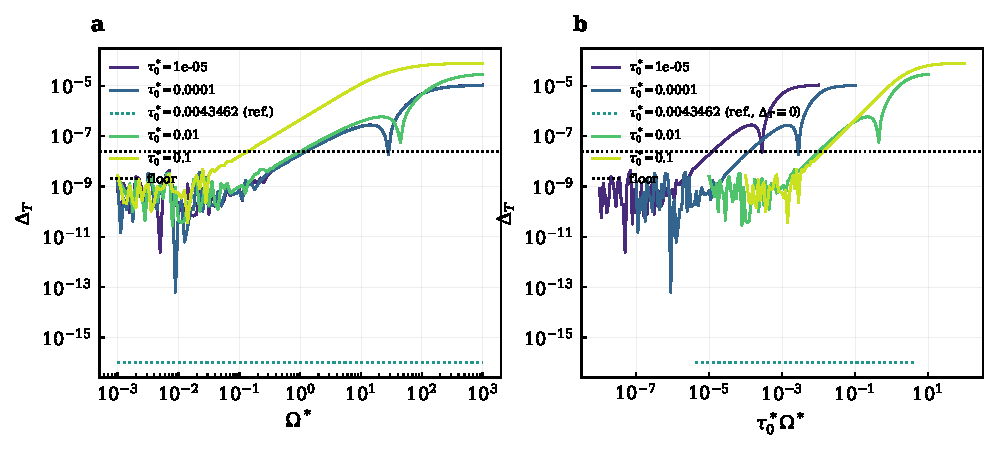
\includegraphics[width=0.98\textwidth]{fig6.pdf}
\caption{Thermal-relaxation sensitivity (model C, isothermal; Study~3). (a)~$\Delta_T=|V(\tau_0^*)-V(\tau_{\mathrm{ref}}^*)|/V(\tau_{\mathrm{ref}}^*)$ versus $\Om^*$ for the five swept $\tau_0^*$ (viridis ramp); the reference $\tau_0^*=4.3462\times10^{-3}$ gives $\Delta_T\equiv0$ by construction (dotted line at the display clip) and is not an independent physical signal. (b)~The same data against the combination $\tau_0^*\Om^*$: for $\tau_0^*\Om^*\gtrsim10^{-2}$ the curves merge onto a common relaxation-controlled branch, while at small $\tau_0^*\Om^*$ they scatter about the floor; the sharp dips are interference nodes where $\Delta_T$ changes sign. Maximum $\Delta_T=7.9\times10^{-5}$ at $\tau_0^*=10^{-1}$, three orders of magnitude above the floor.}
\label{fig:fig6}
\end{figure}

Fig.~\ref{fig:fig6} shows an effect that is present but minor, and its structure is as informative as its size. The oscillation of each $\Delta_T(\Om^*)$ curve about zero (Section~5 records 17--30 sign reversals per curve) indicates an interference-type mechanism: the thermal field perturbs the surface wave in phase at some frequencies and out of phase at others, rather than monotonically stiffening or softening it. The ordering by $\tau_0^*$ --- the largest relaxation time producing the largest deviation --- identifies the relaxation time, not the coupling strength, as the controlling knob within this family of parameters; panel (b) confirms the control variable directly: for $\tau_0^*\Om^*\gtrsim10^{-2}$ all five curves merge onto a single relaxation-controlled branch, while at small $\tau_0^*\Om^*$ they scatter about the floor --- the merged branch is the Lord--Shulman modification acting on the thermal propagator, the scatter is the sub-floor regime. Physically this is expected: the thermoelastic coupling enters through $T_0\beta_1^*\approx2.3\times10^{-3}$, already a small nondimensional number, and the relaxation modifies the thermal response only where $\tau_0^*\Om^*$ is of order unity; at baseline $\tau_0^*$ that condition is met only at the top of the band, where the effect is correspondingly at or below the floor.

\begin{figure}[htbp]
\centering
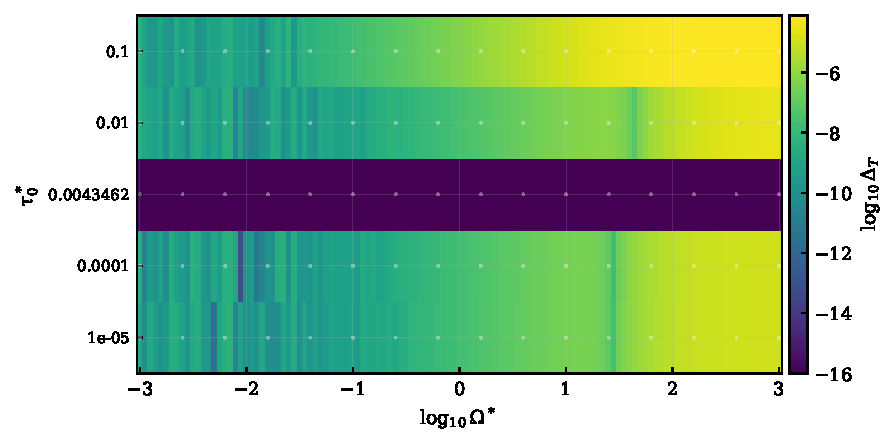
\includegraphics[width=0.98\textwidth]{fig10.pdf}
\caption{Thermal map $\log_{10}\Delta_T(\Om^*,\tau_0^*)$ over the five swept relaxation times (rows) and 121 frequencies (columns); every cell is a computed value (white dots mark a subset of the actual samples), no interpolation. The dark middle row is the reference relaxation time ($\Delta_T\equiv0$, display clip); the resolvable band occupies large $\tau_0^*$ and large $\Om^*$, i.e.\ $\tau_0^*\Om^*\gtrsim1$, consistent with Fig.~\ref{fig:fig6}(b).}
\label{fig:fig10}
\end{figure}

Fig.~\ref{fig:fig10} compresses the same sweep into a map; its message is that the thermal-relaxation effect is confined to a corner of parameter space --- large $\tau_0^*$ and large $\Om^*$ --- exactly where $\tau_0^*\Om^*\gtrsim1$. Everywhere else the thermal channel is a negligible perturbation of the surface branch, which is why the production baseline can be (and is) treated as essentially isothermal-wave physics.

\subsection{Free versus clamped phason boundary (RQ4)}

Replacing the free-phason rows ($H_{xz}=H_{zz}=0$) by clamped rows ($w_x=w_z=0$) over the Study-1 grid (Fig.~\ref{fig:fig7}):
\begin{itemize}
\item \textbf{Model C:} $\Delta V/V\le8.1\times10^{-6}$ (growing monotonically with $\Om$ from $\sim10^{-9}$ at $\Om=10^{-3}$ to $8.06\times10^{-6}$ at $\Om=10^{3}$) --- a small but clearly resolvable boundary effect on a phonon-dominated branch whose phason participation is tiny: clamping the phason acts only through the phonon--phason coupling terms.
\item \textbf{Model A:} clamping the phason \emph{destroys its surface branch}. The computation finds only quasi-static $V^*\to0$ degenerate minima where the clamped phason rows are trivially singular; no comparable finite-speed clamped branch exists. This is reported as a structural result --- the clamped model-A case is excluded from the difference plot rather than represented by an artefact. Physically it is consistent with the branch being phason-dominated ($P_w\approx0.99$): suppressing the phason at the surface removes the very degree of freedom that carries the wave. (The clamped-branch penetration diagnostic still varies strongly, $0.644$--$0.885$ relative, in the recorded raw data.)
\end{itemize}

\begin{figure}[htbp]
\centering
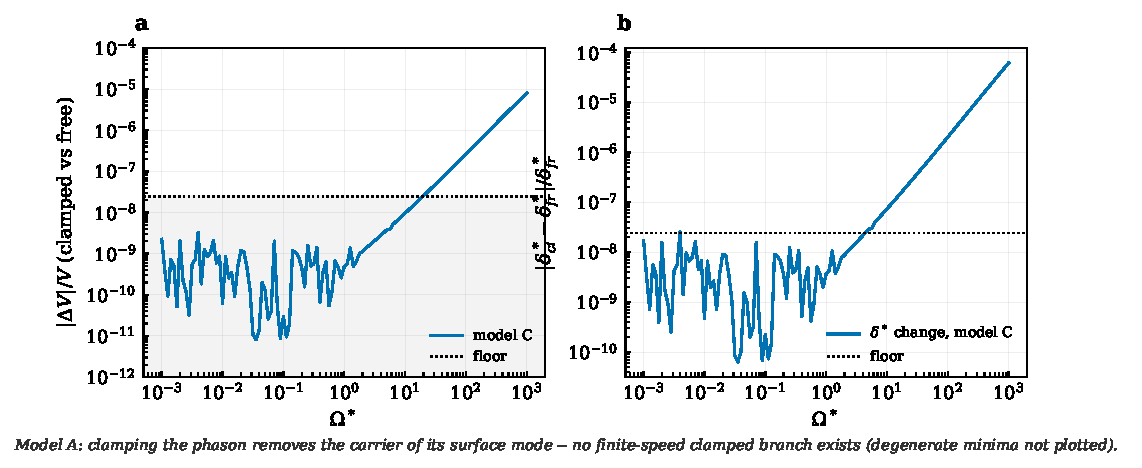
\includegraphics[width=0.98\textwidth]{fig7.pdf}
\caption{Phason boundary condition, clamped ($w_x=w_z=0$) versus free ($H_{xz}=H_{zz}=0$), model C. (a)~$|\Delta V|/V$ growing monotonically from $\sim10^{-9}$ at $\Om^*=10^{-3}$ to $8.1\times10^{-6}$ at $\Om^*=10^{3}$ (sub-floor region shaded). (b)~The corresponding relative change of the dominant penetration depth, of comparable magnitude and likewise growing with $\Om^*$: the boundary condition perturbs the near-surface structure consistently with the speed change. Model A is not plotted: clamping removes the phason carrier of its surface mode and no finite-speed clamped branch exists (degenerate minima excluded; Sections~6.6, 7.6).}
\label{fig:fig7}
\end{figure}

Fig.~\ref{fig:fig7} and the model-A structural finding together answer RQ4, and the asymmetry between the two models is the physical content. Panel (b) shows that the penetration depth of the C branch responds to clamping at the same order and with the same monotone $\Om^*$ growth as the speed: the boundary condition perturbs the near-surface structure of the phonon branch weakly but consistently. For model C the phason boundary condition is a boundary-layer perturbation: the wave is carried by the phonon field, the phason field merely follows it, so pinning the phason at the surface changes the wave speed by at most $8.1\times10^{-6}$ relative, growing with frequency as the coupling terms gain weight. For model A the same boundary operation is catastrophic because it removes the carrier: a branch with $P_w\approx0.99$ is, at the surface, almost pure phason motion, and a clamped phason cannot propagate. The monotonic growth of the model-C curve with $\Om^*$ (no plateau, no saturation inside the band) indicates that the phason boundary sensitivity of the phonon branch is still increasing at $\Om^*=10^{3}$; its extrapolated size at much higher frequency is not established by this study.

\begin{figure}[htbp]
\centering
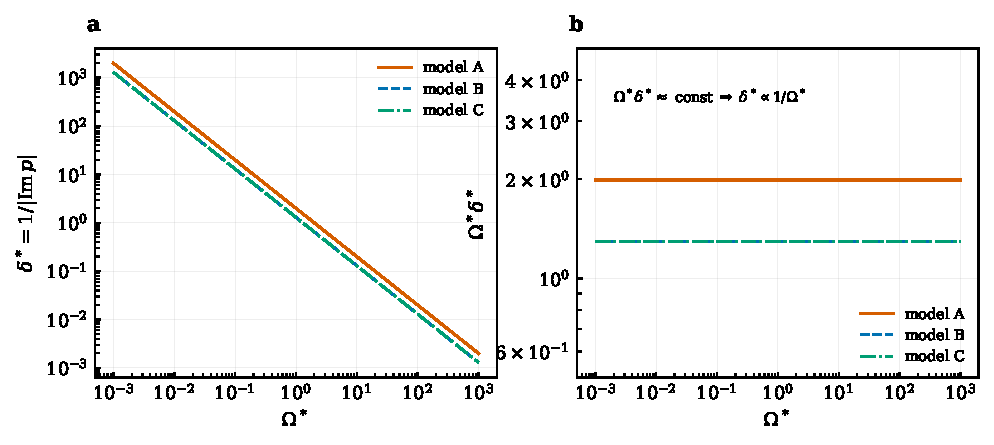
\includegraphics[width=0.98\textwidth]{fig11.pdf}
\caption{Surface localisation. (a)~Dominant penetration depth $\delta^*=1/|\mathrm{Im}\,p|$ versus $\Om^*$ per model (121 production points each); model A penetrates deeper than B/C at equal $\Om^*$, consistent with its slower, softer channel. (b)~The product $\Om^*\delta^*$ is approximately constant ($\approx1.99$ for A, $\approx1.29$ for B/C) across six decades, confirming the classical $1/\Om^*$ localisation of all three branches; $\delta^*$ is depth localisation, not attenuation.}
\label{fig:fig11}
\end{figure}

Fig.~\ref{fig:fig11} completes the branch characterisation: panel (a) shows all three branches localising at the surface with the classical $1/\Om^*$ envelope, and panel (b) verifies the envelope quantitatively --- $\Om^*\delta^*$ is flat at $\approx1.99$ (A) and $\approx1.29$ (B/C) over the whole band --- so every reported mode is a genuine surface wave at every reported frequency. The ordering --- the phason-dominated A branch penetrating deeper than the phonon--Rayleigh branches at the same $\Om^*$ --- is consistent with its slower speed and softer restoring channel; in dimensional terms the A branch probes deeper into the material, which matters for any surface-sensitive measurement interpretation.

\section{Discussion}

\subsection{What controls the surface branch: dynamical class, not parameters}

The organising result of this study is that in a 2D hexagonal piezoelectric thermoelastic quasicrystal half-space the \emph{dynamical class} of the phason field --- inertial, diffusive, or telegraph-type --- decides which surface branch the free surface supports, while every continuous parameter explored (frequency over six decades, friction over four decades, relaxation time over four decades, phason boundary condition) modifies that branch only perturbatively. Model A's branch ($V^*\approx0.311$, $P_w\approx0.991$) and the B/C branch ($V^*\approx0.466$, phonon-dominated) are not two states of one mode connected by parameter variation; within the investigated ranges they are distinct modes selected by the structure of the phason balance law. The modelling implication is direct: before any quantitative surface-wave computation on a quasicrystal, the phason dynamic law must be fixed --- it is a branch-selection decision, not a refinement.

\subsection{Physical meaning of the inertial (model A) branch}

Why does phason inertia create a distinct surface mode? In model A the phason field carries kinetic energy $\tfrac12\rw|\dot w|^2$, so surface-localised phason oscillation can balance the phason stiffness $K_3$ against inertia, in the same way that phonon inertia balances $C_{66}$ in a Rayleigh wave. The resulting branch sits at $V^*\approx\sqrt{K_3^*}=0.316$ scaled down by coupling --- the computed $0.31072662$ is $1.7\%$ below $\sqrt{K_3^*}$, and the documented near-grazing degeneracy of the branch (the $V^*<\sqrt{K_3^*}$ requirement for five roots, Section~3.6) is the surface-wave expression of that phason-shear threshold. The branch is almost pure phason ($P_w\approx0.99$) because the phonon--phason coupling $R_6^*=0.0125$ is weak relative to the phason channel. A caution attaches to this interpretation: $\rw=\rho$ is a declared surrogate identification (no independent phason mass density exists in the literature), so the \emph{existence} of the branch is a property of the model class, while its \emph{speed} inherits the surrogate inertia scale.

\subsection{Physical meaning of the diffusive (model B) branch: slaved phasons}

In model B the phason field has no independent dynamics: its balance law is first order in time, so at frequency $\om$ the phason responds with amplitude slaved to the phonon strain through a dissipative propagator $\propto(\mathrm{i}\om\Dw)^{-1}$. The computed participation numbers are the quantitative form of this slaving: $P_w$ between $1.7\times10^{-13}$ and $1.8\times10^{-5}$ across the band --- the phason follows the phonon field as a small, dissipatively lagging shadow. The surface wave is therefore the classical Rayleigh wave dressed by phason compliance: the quasi-static verification value $0.9326028\,v_S$ exceeds the decoupled Rayleigh ratio by $7.7\times10^{-5}$ precisely by this dressing. No independent phason inertia exists in the model, so no phason branch exists --- a negative result that follows structurally from the degree count ($\deg_\om\det M=8$ versus 10).

\subsection{Model C, the ratio $\Om/\Om_c$, and what the maps show}

Model C contains both mechanisms with the competition parameter $\Om/\Om_c$, $\Om_c=\Dw^*/\rw^*$. The production data give a consistent, bounded reading: (i)~at baseline $\Om_c=11467.5$, the whole band has $\Om/\Om_c\le8.7\times10^{-2}$, the inertial term is negligible, and C is numerically the same as B (Section~6.1); (ii)~in the controlled-friction study the $\Delta_{BC}$ difference grows as the friction decreases, reaching $5.0\times10^{-3}$ at $D_w^*=1$, i.e.\ the difference is a smooth perturbative function of $\Om/\Om_c$; (iii)~the resolvable wedge of Fig.~\ref{fig:fig9} opens at frequencies \emph{below} the bare $\Om_c$ line, because surface-wave separability depends on how the phason propagator modifies the \emph{branch minimum}, not on the bulk phason operator alone. The distinction that must be preserved in any summary of this study is therefore between the \emph{operator} crossover $\Om_c$ (a model property, drawn as a reference line) and the \emph{resolution boundary} of the $\Delta_{BC}$ wedge (a property of the solver's floor); the baseline window contains neither an operator crossover nor a claimed material transition.

\subsection{Why the thermal effect is small}

Three parameter-set facts, each verifiable from Table~\ref{tab:params} and \eqref{eq:starred}, explain the magnitude $\max\Delta_T=7.9\times10^{-5}$: (i)~the thermoelastic coupling group $T_0\beta_1^*=2.3\times10^{-3}$ is intrinsically small, so the thermal channel is a weak perturbation of the elastic problem before relaxation is even considered; (ii)~the relaxation acts through $\tau_0^*\Om^*$, and at baseline $\tau_0^*=4.3\times10^{-3}$ this product reaches unity only at $\Om^*\approx230$; (iii)~the Lord--Shulman modification of the thermal propagator is itself significant only for $\tau_0^*\Om^*\gtrsim1$. All three conditions coincide only in the upper corner of the swept $(\Om^*,\tau_0^*)$ plane, which is exactly where Fig.~\ref{fig:fig10} places the resolvable band. This explanation is a property of the \emph{declared parameter set}, not a universal statement: a material with stronger $\beta_1$, larger $T_0$, or a relaxation time near the wave period would show a correspondingly larger thermal effect. What is universal within this formulation is the \emph{mechanism}: thermal relaxation enters the surface wave through the product $\tau_0^*\Om^*$ and the coupling group, and nowhere else.

\subsection{Phason boundary conditions: what free and clamped constrain}

The free condition $H_{xz}=H_{zz}=0$ is the natural condition for a surface at which the quasiperiodic structure may re-arrange without phason-stress cost; it is the condition adopted for 2D hexagonal half-spaces in the literature \cite{wang2015}. The clamped condition $w_x=w_z=0$ pins the quasiperiodic tiling at the surface --- physically, a surface at which atomic re-arrangements are inhibited (for instance by a coherent epitaxial overlayer or by pinning sites). The two boundary conditions therefore bracket the range of physical surface preparations. The asymmetric response of the models is the physically interesting content: the phonon-dominated branch (C) is nearly indifferent ($\le8.1\times10^{-6}$) because its surface energy is carried by phonon traction, while the phason-dominated branch (A) cannot exist at all under clamping --- its carrier is removed at the boundary. The model-A clamped degeneracy must not be reinterpreted as a finite-speed branch at another speed: the recorded data contain only quasi-static degenerate minima, and the penetration diagnostic of those minima ($0.644$--$0.885$ relative variation) characterises a degenerate set, not a wave.

\subsection{Penetration structure and near-surface character}

All reported branches decay as $\mathrm{e}^{-z/\delta^*}$ with $\delta^*\propto1/\Om^*$ (Fig.~\ref{fig:fig11}), so the surface character of the modes is robust across the band. Two features have modelling consequences. First, the A branch's larger $\delta^*$ means a phason-dominated surface mode probes a deeper layer of material than the phonon--Rayleigh mode at the same frequency; a surface measurement sensitive to a depth $d$ would couple preferentially to the A branch at $\Om^*\lesssim1/\delta^*_{\text{target}}$. Second, the monotone shrinkage of $\delta^*$ with $\Om^*$ means that at the top of the band all branches are confined to a surface layer of nondimensional thickness $\sim10^{-3}$; the homogeneous half-space assumption of this study is then a statement about that thin layer only, and any near-surface grading, coating, or damage within it would affect the reported speeds --- such effects are outside the present homogeneous formulation and are flagged here rather than estimated.

\subsection{Relation to the 1D hexagonal surface-wave literature}

The 1D hexagonal studies (Section~1.4) share the surface-matrix methodology and several physical messages with this work: phason coupling lowers the surface speed relative to the decoupled elastic value, and piezoelectricity adds an electrical branch structure in suitable configurations. Two differences are structural rather than numerical and prevent transplanting their results. (i)~Field content: the 1D sagittal problem carries one phason component, the 2D hexagonal problem carries two plus the shear asymmetry $H_{xz}\neq H_{zx}$ --- which enters the depth polynomial through the identity \eqref{eq:A1ident} and modifies the fifth boundary row. (ii)~Surface condition: the 1D free surface releases a single phason traction, the 2D surface releases two; the clamped-phason study of Section~6.6 (which destroys the model-A branch) has no 1D analogue in the surveyed literature. Within the surveyed literature this is the first surface-wave analysis of the 2D hexagonal class that carries all three phason dynamic models; the comparison to 1D results is qualitative, because the formulations are different.

\subsection{Limitations}

The limitations are stated explicitly:
\begin{enumerate}
\item \textbf{Surrogate/composite parameters.} The parameter set is a composite literature table with declared surrogates ($\rho=4180$~kg/m$^3$, $c_e=500$~J/(kg\,K)); $\rw=\rho$ is a declared identification; $k_{11}=6$~W/(m\,K) conflicts with 5.3 in the same source (unresolved, declared). No single fully characterised 2D hexagonal quasicrystal specimen underlies the set; results are model statements, not material predictions.
\item \textbf{No experimental validation.} Nothing in this paper is experimentally calibrated or verified; in particular, no observability in any specific experiment is claimed.
\item \textbf{Semi-analytical homogeneous half-space.} No layering, grading, imperfection, or finite-depth effects; no independent discretisation-based cross-check (the method of this paper is semi-analytical by design; verification rests on the classical limits, symbolic identities, and two-path consistency of Section~5).
\item \textbf{Configuration-I restriction.} $y$-independence, $u_y=0$, exact decoupling of the electric potential; other cuts invalidate the decoupling.
\item \textbf{2D hexagonal scope.} Conclusions do not extend to 1D hexagonal or icosahedral quasicrystals, whose constitutive structures differ.
\item \textbf{Numerical resolution.} A/B/C differences at or below $\e_\Delta=1.13\times10^{-8}$ are indistinguishable, not zero; the resolution floor is benchmarked, not asserted.
\item \textbf{Model-A clamped degeneracy.} No comparable clamped branch exists for model A; no finite clamped speed is reported for it.
\item \textbf{Reference-line interpretation.} $\Om_c=D_w^*/\rw^*$ in Figs.~\ref{fig:fig9} is a reference line, not a validated transition.
\item \textbf{Singular model limits.} The $\Dw\to0$ limit is non-uniform in $\Om$ (Section~5.3); limit statements carry their verified $\Om$ ranges.
\item \textbf{Parameter ranges.} All statements hold within the swept ranges of Table~\ref{tab:nondim}; extrapolation beyond them is not supported by this study.
\end{enumerate}

\section{Conclusions}

\begin{enumerate}
\item \textbf{Formulation.} A complete semi-analytical surface-wave formulation for 2D hexagonal piezoelectric thermoelastic quasicrystals (Laue class~10) has been established and verified. \emph{Physical meaning:} the sagittal problem is a five-field boundary-value problem whose depth structure is a tenth-degree matrix pencil preserving the phason-stress asymmetry $H_{xz}\neq H_{zx}$. \emph{Modelling implication:} the formulation provides an exact, discretisation-free baseline against which layered, graded, or discretised treatments of this material class can be checked.
\item \textbf{Verification.} Classical limits are reproduced to machine precision ($v_P/v_0=1$, $v_S/v_0=1/2$; Rayleigh ratio to $1.1\times10^{-11}$), symbolic identities hold exactly, and the model limits C$\to$A and C$\to$B are verified on the full grid ($\le3.3\times10^{-9}$) with branch-identity-verified continuation. \emph{Physical meaning:} model C genuinely interpolates between the inertial and diffusive classes; the retained $10^{-8}$ evidence curve quantifies the smooth non-uniformity of the singular $\Dw\to0$ limit below $\Om\approx0.32$. \emph{Modelling implication:} telegraph-type phason models can be used safely as one-parameter families, with the limit statements carrying their verified $\Om$ ranges.
\item \textbf{Branch selection at baseline (RQ1).} At baseline friction ($D_w^*=11467.5$, $\Om_c\gg\Om_{\max}$), model A supports a phason-dominated branch at $V^*\approx0.311$ ($P_w\approx0.99$), while models B and C both support the phonon--Rayleigh branch at $V^*\approx0.466$, mutually indistinguishable over 95/121 grid points within the benchmarked floor. \emph{Physical meaning:} inertial phasons carry their own surface mode; dissipative phasons are slaved to the phonon field. \emph{Modelling implication:} the choice of phason dynamic law is a branch-selection decision that must be made before quantitative work; diffusive versus telegraph is not such a decision at baseline friction.
\item \textbf{Controlled friction (RQ2).} At $D_w^*\le10^{0}$ the B--C difference reaches $5.0\times10^{-3}$ relative and exceeds the floor over nearly the whole band; at baseline $D_w^*$ the two models agree to $\le1.25\times10^{-7}$ across the map. The operator crossover $\Om_c=D_w^*/\rw^*$ is a reference line; no transition in the surface-wave data is claimed at it. \emph{Physical meaning:} the diffusive/telegraph distinction is a perturbative effect controlled by $\Om/\Om_c$, not a mode transition. \emph{Modelling implication:} friction values and frequency bands must be stated together when comparing phason dynamic models; a difference observed at low friction must not be extrapolated to high friction.
\item \textbf{Thermal relaxation (RQ3).} Lord--Shulman relaxation produces a weak, resolvable surface-wave effect ($\max\Delta_T=7.9\times10^{-5}$ at the largest swept $\tau_0^*$, three orders above the floor); near baseline $\tau_0^*$ the effect is at or below the floor. \emph{Physical meaning:} thermal relaxation acts through $\tau_0^*\Om^*$ and the small coupling group $T_0\beta_1^*$, so it matters only in the upper corner of the swept plane. \emph{Modelling implication:} within this parameter set, surface-wave predictions are robust to the choice of $\tau_0^*$ near baseline; a thermally refined treatment pays off only at large $\tau_0^*\Om^*$.
\item \textbf{Phason boundary conditions (RQ4).} Clamping the phason changes the model-C speed by at most $8.1\times10^{-6}$ relative and destroys the model-A surface branch entirely. \emph{Physical meaning:} the phonon branch stores its surface energy in phonon traction, the phason branch in phason motion --- pinning the phason removes the latter's carrier. \emph{Modelling implication:} phason boundary conditions are a secondary parameter for phonon-dominated waves but a first-order modelling decision whenever a phason-dominated branch is possible (low friction or inertial phason models).
\end{enumerate}
These conclusions hold for the declared parameter set and are bounded by the numerical-resolution floor and the stated limitations (Section~7.9); in particular, they are not extended to specific materials, layered structures, other propagation configurations, or experimentally measured quantities.

\section*{Data and code availability}
The numerical results were generated using the semi-analytical surface-wave implementation described in this work. The computational scripts, input parameters, raw numerical data, validation records, and figure-generation materials required to reproduce the reported results are provided in the accompanying reproducibility package (submitted as supplementary material); checksums and provenance metadata are recorded in that package's manifest. [PUBLIC ARCHIVE IDENTIFIER TO BE INSERTED IF/WHEN DEPOSITED.]

\section*{Declarations}
{\sloppypar\noindent\textbf{Funding:} [FUNDING INFORMATION TO BE INSERTED]. \textbf{Conflict of interest:} [CONFLICT-OF-INTEREST STATEMENT TO BE INSERTED]. \textbf{Author contributions:} [TO BE INSERTED]. No human or animal subjects are involved.\par}

\begin{thebibliography}{47}\small
\bibitem{shechtman1984} Shechtman, D., Blech, I., Gratias, D., Cahn, J.W.: Metallic phase with long-range orientational order and no translational symmetry. \emph{Phys. Rev. Lett.} \textbf{53}, 1951--1953 (1984). DOI 10.1103/PhysRevLett.53.1951
\bibitem{levine1984} Levine, D., Steinhardt, P.J.: Quasicrystals: a new class of ordered structures. \emph{Phys. Rev. Lett.} \textbf{53}, 2477--2480 (1984). DOI 10.1103/PhysRevLett.53.2477
\bibitem{janot1994} Janot, C.: \emph{Quasicrystals: A Primer}, 2nd edn. Oxford University Press, Oxford (1994)
\bibitem{steurer2009} Steurer, W., Deloudi, S.: \emph{Crystallography of Quasicrystals: Concepts, Methods and Structures}. Springer Series in Materials Science, vol.~126. Springer, Berlin/Heidelberg (2009). DOI 10.1007/978-3-540-68292-9
\bibitem{bak1985} Bak, P.: Symmetry, stability, and elastic properties of icosahedral incommensurate crystals. \emph{Phys. Rev. B} \textbf{32}, 5764--5772 (1985). DOI 10.1103/PhysRevB.32.5764
\bibitem{levin1985} Levin, D., Lubensky, T.C., Ostlund, S., Ramaswamy, S., Steinhardt, P.J., Toner, J.: Elasticity and dislocations in pentagonal and icosahedral quasicrystals. \emph{Phys. Rev. Lett.} \textbf{54}, 1520--1523 (1985). DOI 10.1103/PhysRevLett.54.1520
\bibitem{socolar1986} Socolar, J.E.S., Lubensky, T.C., Steinhardt, P.J.: Phonons, phasons, and dislocations in quasicrystals. \emph{Phys. Rev. B} \textbf{34}, 3345--3360 (1986). DOI 10.1103/PhysRevB.34.3345
\bibitem{lubensky1985} Lubensky, T.C., Ramaswamy, S., Toner, J.: Hydrodynamics of icosahedral quasicrystals. \emph{Phys. Rev. B} \textbf{32}, 7444--7452 (1985). DOI 10.1103/PhysRevB.32.7444
\bibitem{ding2000} Ding, D.H., Hu, C.Z., Wang, R.H.: Symmetry groups, physical property tensors, elasticity and dislocations in quasicrystals. \emph{Rep. Prog. Phys.} \textbf{63}, 1--39 (2000). DOI 10.1088/0034-4885/63/1/201
\bibitem{fan2011} Fan, T.: \emph{Mathematical Theory of Elasticity of Quasicrystals and Its Applications}. Springer, Berlin/Heidelberg (2011). DOI 10.1007/978-3-642-14643-5
\bibitem{fan2004amr} Fan, T.Y., Mai, Y.W.: Elasticity theory, fracture mechanics, and some relevant thermal properties of quasi-crystalline materials. \emph{Appl. Mech. Rev.} \textbf{57}, 325--343 (2004)
\bibitem{deboissieu2012} de Boissieu, M.: Phonons, phasons and atomic dynamics in quasicrystals. \emph{Chem. Soc. Rev.} \textbf{41} (2012) [page range not independently verified in this audit]
\bibitem{francoual2003} Francoual, S., et al.: Phason fluctuations and the dynamical structuration of a quasicrystal. \emph{Phys. Rev. Lett.} \textbf{91}, 225502 (2003). As cited in \cite{agiasofitou2014}
\bibitem{chellappan2015} Chellappan, V., Gopalakrishnan, S., Mani, V.: Wave propagation of phonon and phason displacement modes in quasicrystals: determination of wave parameters. \emph{J. Appl. Phys.} \textbf{117}, 054905 (2015). DOI 10.1063/1.4907212
\bibitem{agiasofitou2014} Agiasofitou, E.C., Lazar, M.: The elastodynamic model of wave-telegraph type for quasicrystals. \emph{Int. J. Solids Struct.} \textbf{51}, 923--929 (2014). DOI 10.1016/j.ijsolstr.2013.11.016
\bibitem{agiasofitou2014mrc} Agiasofitou, E., Lazar, M.: On the equations of motion of dislocations in quasicrystals. \emph{Mech. Res. Commun.} \textbf{57}, 27--33 (2014)
\bibitem{lazar2014pm} Lazar, M., Agiasofitou, E.: Fundamentals in generalized elasticity and dislocation theory of quasicrystals: Green tensor, dislocation key-formulas and dislocation loops. \emph{Philos. Mag.} \textbf{94}, 4080--4101 (2014)
\bibitem{agiasofitou2023} Agiasofitou, E., Lazar, M.: On the constitutive modelling of piezoelectric quasicrystals. \emph{Crystals} \textbf{13}, 1652 (2023). DOI 10.3390/cryst13121652
\bibitem{barnett1985} Barnett, D.M., Lothe, J.: Free surface (Rayleigh) waves in anisotropic elastic half-spaces: the surface impedance method. \emph{Proc. R. Soc. Lond. A} \textbf{402}, 135--152 (1985)
\bibitem{bleustein1968} Bleustein, J.L.: A new surface wave in piezoelectric materials. \emph{Appl. Phys. Lett.} \textbf{13}, 412 (1968). DOI 10.1063/1.1652495
\bibitem{gulyaev1969} Gulyaev, Y.V.: Electroacoustic surface waves in solids. \emph{Sov. Phys. JETP} \textbf{9}, 37 (1969)
\bibitem{lord1967} Lord, H.W., Shulman, Y.: A generalized dynamical theory of thermoelasticity. \emph{J. Mech. Phys. Solids} \textbf{15}, 299--309 (1967). DOI 10.1016/0022-5096(67)90024-5
\bibitem{green1972} Green, A.E., Lindsay, K.A.: Thermoelasticity. \emph{J. Elasticity} \textbf{2}, 1--7 (1972)
\bibitem{chandrasekharaiah1986} Chandrasekharaiah, D.S.: Thermoelasticity with second sound --- a review. \emph{Appl. Mech. Rev.} \textbf{39}, 355--376 (1986). DOI 10.1115/1.3143705
\bibitem{chandrasekharaiah1998} Chandrasekharaiah, D.S.: Hyperbolic thermoelasticity: a review of recent literature. \emph{Appl. Mech. Rev.} \textbf{51}, 705--729 (1998)
\bibitem{ignatzak2009} Ignaczak, J., Ostoja-Starzewski, M.: \emph{Thermoelasticity with Finite Wave Speeds}. Oxford University Press, Oxford (2009)
\bibitem{chadwick1970} Chadwick, P., Seet, L.T.C.: Wave propagation in a transversely isotropic heat-conducting elastic material. \emph{Mathematika} \textbf{17}(2) (1970). DOI 10.1112/S002557930000293X
\bibitem{yang1994prb} Yang, W.G., Ding, D.H., Hu, C.Z., Wang, R.H.: \emph{Phys. Rev. B} \textbf{49}, 12656 (1994). As cited in the reference list of \cite{wang2021} for the symmetry relations of its eq.~(7); the relations are re-derived independently in the present formulation
\bibitem{yang2014} Yang, L., Zhang, L., Song, F., Gao, Y.: General solutions for three-dimensional thermoelasticity of two-dimensional hexagonal quasicrystals and an application. \emph{J. Therm. Stresses} \textbf{37}, 363--379 (2014). DOI 10.1080/01495739.2013.869149
\bibitem{wang2015} Wang, T., Li, X.Y., Zhang, X., M\"uller, R.: Fundamental solutions in a half space of two-dimensional hexagonal quasicrystal and their applications. \emph{J. Appl. Phys.} \textbf{117}, 154904 (2015). DOI 10.1063/1.4918535
\bibitem{li2017} Li, X.-Y., Wang, Y.-W., Li, P.-D., Kang, G.-Z., M\"uller, R.: Three-dimensional fundamental thermo-elastic field in an infinite space of two-dimensional hexagonal quasi-crystal with a penny-shaped/half-infinite plane crack. \emph{Theor. Appl. Fract. Mech.} \textbf{88}, 18--30 (2017). DOI 10.1016/j.tafmec.2016.11.005
\bibitem{li2024ijhmt} Li, Y., Tang, S., Ren, J., Yan, S., Zhao, M.: Thermoelastic fracture of two-dimensional hexagonal quasicrystal media weakened by a penny-shaped crack subjected to uniformly antisymmetric heat fluxes. \emph{Int. J. Heat Mass Transf.} \textbf{235}, 126202 (2024). DOI 10.1016/j.ijheatmasstransfer.2024.126202
\bibitem{wang2021} Wang, W., Li, C., Zhou, Y.-T.: Thermo-electric response in 2D hexagonal QC exhibiting piezoelectric effect. \emph{Z. Angew. Math. Mech.} \textbf{101}, e201900212 (2021). DOI 10.1002/zamm.201900212
\bibitem{li2024ejma} Li, Y., Tang, S., Ren, J., Yan, S., Zhao, M.: Analytical solutions to Mode I penny-shaped crack problems in two-dimensional hexagonal quasicrystals with piezoelectric effect. \emph{Eur. J. Mech. A/Solids} \textbf{108}, 105425 (2024). DOI 10.1016/j.euromechsol.2024.105425
\bibitem{zhou2019ejma} Zhou, Y.B., Li, X.F.: Fracture analysis of an infinite 1D hexagonal piezoelectric quasicrystal plate with a penny-shaped dielectric crack. \emph{Eur. J. Mech. A/Solids} \textbf{76}, 224--234 (2019)
\bibitem{hosseini2019} Hosseini, S.M., Bavi, O., Bavi, H., Eslami, M.R.: A novel meshless method based on a local integral equation (LIE) for two-dimensional thermoelasticity of decagonal quasicrystals subjected to thermal shock. \emph{Appl. Math. Model.} \textbf{66}, 275--295 (2019). DOI 10.1016/j.apm.2018.09.024
\bibitem{lizhou2024} Li, Y., Zhou, Y.: Dynamic response of a piezoelectric quasicrystal rod with the generalized thermoelasticity. \emph{Acta Mech.} \textbf{235}, 323--335 (2024). DOI 10.1007/s00707-023-03747-4
\bibitem{zhang2023cryst} Zhang, B., Tu, H., Li, L., Yu, J., Dai, J.: Rayleigh waves propagating in the functionally graded one-dimensional hexagonal quasicrystal half-space. \emph{Crystals} \textbf{13}, 1205 (2023). DOI 10.3390/cryst13081205
\bibitem{zhang2024amm} Zhang, B., Tu, H., Chen, W., Yu, J., Elmaimouni, L.: A coupled Legendre--Laguerre polynomial method with analytical integration for the Rayleigh waves in a quasicrystal layered half-space with an imperfect interface. \emph{Appl. Math. Mech.-Engl. Ed.} \textbf{45}, 1539--1556 (2024). DOI 10.1007/s10483-024-3145-8
\bibitem{zhang2025zamm} Zhang, B., Tu, H., Li, L., Han, H., Yu, J., Elmaimouni, L., Yang, X.: Rayleigh and Love waves in 1-D hexagonal piezoelectric quasicrystal layered half-space structures with an imperfect interface. \emph{Z. Angew. Math. Mech.} (2025). DOI 10.1002/zamm.70114
\bibitem{zhang2021amss} Zhang, B., Yu, J., Zhang, X., Wang, X.: Guided waves in the multilayered one-dimensional hexagonal quasi-crystal plates. \emph{Acta Mech. Solida Sin.} \textbf{34}, 91--103 (2021)
\bibitem{zhang2021acta} Zhang, B., Yu, J.G., Zhang, X.M., Elmaimouni, L.: Guided wave propagating in a 1-D hexagonal piezoelectric quasi-crystal plate. \emph{Acta Mech.} (2021). DOI 10.1007/s00707-020-02811-7
\bibitem{feng2024amm} Feng, X., Ke, L., Gao, Y.: Love wave propagation in one-dimensional piezoelectric quasicrystal multilayered nanoplates with surface effects. \emph{Appl. Math. Mech.-Engl. Ed.} \textbf{45}, 619--632 (2024)
\bibitem{ma2023zamp} Ma, Y., Zhou, Y., Yang, J., Zhang, X., Wang, X., Ding, S.: Interface crack behaviors disturbed by Love waves in a 1D hexagonal quasicrystal coating--substrate structure. \emph{Z. Angew. Math. Phys.} \textbf{74}, 61 (2023). DOI\linebreak 10.1007/s00033-023-01947-5
\bibitem{yang2022zamm} Yang, J., Wang, X., Ding, S., et al.: Scattering of SH wave by a crack in a functionally graded one-dimensional hexagonal piezoelectric quasicrystal. \emph{Z. Angew. Math. Mech.} \textbf{103}(2), e202200071 (2022). DOI 10.1002/zamm.202200071
\bibitem{shaonan2025actamech} Li, S., Ding, S., Ma, Y., et al.: SH wave scattering by a circular arc-shaped nano-hole located within the half-plane boundary of one-dimensional hexagonal quasicrystals. \emph{Acta Mech.} (2025). DOI 10.1007/s00707-025-04361-2
\bibitem{wang2024sem} Wang, H.T., Guo, J.H.: Nonlocal bending, vibration and buckling of one-dimensional hexagonal quasicrystal layered nanoplates with imperfect interfaces. \emph{Struct. Eng. Mech.} \textbf{89}, 557--570 (2024)
\end{thebibliography}

\end{document}
